\iftrue
    \PassOptionsToPackage{hyphens}{url}
    \documentclass[10pt,a4paper]{article}
    \usepackage[text={6.5in,10in},centering]{geometry}    
    \usepackage{url}
    \usepackage{doi}
    \usepackage{longtable}
    \usepackage{color}
    \usepackage{amsmath,amssymb}
    \usepackage{fancyhdr}
    \usepackage{graphicx}
\usepackage{amssymb}
\usepackage{epstopdf}
    \def\httpURL#1{\href{http://#1}{\textcolor{blue}{#1}}}
    \def\LONGhttpURL#1#2{\href{http://#1}{\textcolor{blue}{#2}}}    
    \input paper-seb-macros.tex
\fi

\makeatletter
      \renewcommand{\thefootnote}{\arabic{footnote}}
      \let\oldbibcite=\bibcite
      % example: \bibcite{bad-code}{{31}{2020}{{Richards and Boudnik}}{{Richards and Boudnik}}}
      \newcount\mainNumberOfReferences \mainNumberOfReferences=0
      \def\bibcite#1#2{\global\advance\mainNumberOfReferences by 1\oldbibcite{#1}{#2}}
      \input paper-seb-main.aux 
      %\resetlinenumber[\MainPaperLastLine]
	  \let\bibcite=\oldbibcite
\makeatother

\input generated/page-lengths.tex

\begin{document}

\title{\textbf{\supplement}\vskip 2ex \mytitle\vskip 2ex}

\author{Harold Thimbleby, \texttt{harold@thimbleby.net}}

%\orcid{0000-0003-2222-4243}

\def\href#1{#1}

\maketitle
\pagestyle{fancy}

% pageref gives us a hyperlink which looks unsightly, so we do it this way...
\makeatletter
\def\rememberpage{\immediate\write\@auxout{\bslash gdef\bslash SupplementalLastPage{\thepage}}}
\makeatother

\rfoot{\supplement\ \thepage/\SupplementalLastPage}
\lfoot{\today}
\cfoot{}
\lhead{}
\rhead{}
\renewcommand{\headrulewidth}{0pt}
\renewcommand{\footrule}{\hrule height 2pt \vspace{2mm}}
\thispagestyle{empty}

% this will be used to save cross references that can be used in the main paper too
\newwrite\infofileForMain
\immediate\openout\infofileForMain=generated/info-for-main.tex

%\makeatletter
%% saves name-value pairs in both the supplementary material .aux file and the info for the main file
%\def\remembernamevalue#1#2{%
%	\immediate\write\@auxout{\@backslashchar gdef\@backslashchar #1{#2}}%
%	\immediate\write\infofileForMain{\@backslashchar gdef\@backslashchar #1{#2}}%
%}
%\makeatother

\input generated/info-for-supplement.tex
\newwrite\infofileForSupplement
\immediate\openout\infofileForSupplement=generated/info-for-supplement.tex

\def\dotalph#1{\ifnum\csname c@#1\endcsname>0 .\alph{#1}\fi}

% writing to the aux file, this file generates labels like
% \newlabel{supplementary-best-practice}{{2}{5}{Software engineering best practice}{section.2}{}}
% whereas the main file using IEEEtrans class generates
% \newlabel{table-summary}{{I}{5}} or \newlabel{jvs-policy}{{V}{4}} etc

\makeatletter
\def\globalLabel#1{% we also need journal code-policies to be used in the main paper...
\typeout{Global globalLabel: #1}%
\immediate\write\infofileForMain{\bslash newlabel{#1}{{\arabic{section}}{\thepage}{DUMMYA}{DUMMYB}{DUMMYC}}}
% as well as in the current document....
\immediate\write\@auxout{\bslash newlabel{#1}{{\bslash arabic{section}\dotalph{subsection}}{\thepage}{AAA}{BBB}{CCC}}}
}
\def\globalTableLabel#1{% we also need journal code-policies to be used in the main paper...
\typeout{Global globalTableLabel: #1}%
\immediate\write\infofileForMain{\bslash newlabel{#1}{{\arabic{table}}{\thepage}{DUMMYA}{DUMMYB}{DUMMYC}}}
% as well as in the current document....
\immediate\write\@auxout{\bslash newlabel{#1}{{\bslash arabic{table}\dotalph{subsection}}{\thepage}{AAA}{BBB}{CCC}}}
}
\def\globalLabelValue#1#2{% we also need journal code-policies to be used in the main paper...
\typeout{Global globalLabelValue: #1 := #2}%
\immediate\write\infofileForMain{\bslash newlabel{#1}{{#2}{\thepage}{AAA}{BBB}{CCC}}}
}
\makeatother

% start supplementary material's page counters to continue on from the paper's page numbering
\setcounterpageref{page}{LastPage}
\addtocounter{page}{1} % otherwise we start with the same page that the main paper ended on (we want to be on the next page:-)!

%\setcounter{section}{0}
\setcounter{section}{\continueSectionNumbers}
\def\n#1{{\sf\bfseries ({#1})}}

\newdimen \www 
\setbox0=\hbox{\n{viii}~}
\www=\wd0 \advance \www by .4em
\def\nnInContents#1#2{\hbox to \www {\hfill\n{#1}~\hskip .4em} #2\\}

\setbox0=\hbox{\sfdefault\large(00)}
\newdimen\howwide \howwide=\wd0 \howwide=2.5em

\def\sec#1#2#3{\setbox0=\hbox{\n{#1}~~}\leftskip \wd0
%\begin{flushleft}
\subsubsection*{\setbox0=\hbox{\n{#1}~~}\hskip -\wd0\copy0 \bfseries
\immediate\write\minicontentsfile{\bslash nnInContents{#1}{#3}}%
{#2}\starredsubsectioncontents{\hbox to \howwide{\hfill (#1)} #3}}
%\end{flushleft}
\leavevmode
\vskip 1ex
\par\leftskip 0in}

\def\highlightsec#1#2#3{\sec{#1}{{#2}}{{#3}}}
\def\highlightmysubsection#1{\subsection{{#1}}\subsectioncontents{{#1}}}
\def\changemysubsection#1{\subsection{{#1}}\subsectioncontents{{#1}}}
\def\changemysection#1{\vskip 2ex\section{{#1}}\sectioncontents{{#1}}}
\def\highlightmysection#1{\section{{#1}}\sectioncontents{{#1}}}
\def\mysection#1{\section{#1}\sectioncontents{#1}}
\def\mysubsection#1{\subsection{#1}\subsectioncontents{#1}}

\makeatletter
\let \bslash = \@backslashchar
\makeatother

\def\sectioncontents#1{\immediate\write\contentsfile{\bslash contents{\arabic{section} #1}{\thepage}}}
\def\subsectioncontents#1{\immediate\write\contentsfile{\bslash subcontents{\alph{subsection}\ #1}{\thepage}}}
\def\starredsubsectioncontents#1{\immediate\write\contentsfile{\bslash subcontents{#1}{\thepage}}}

\noindent\vbox{% The table of contents
\def\contents#1#2{\vskip 0mm \noindent{\bfseries #1} \dotfill\ #2\\}
\def\subcontents#1#2{\hbox to 1em{}{#1} \dotfill\ #2\\}
\noindent\small
\input generated/supplementary.toc
}

\newwrite\contentsfile
\immediate\openout\contentsfile=generated/supplementary.toc

\newpage
\begin{center}
\emph{Pagination, section, and citation numbering continues from the main paper}
\end{center}
\mysection{Further issues for Software Engineering Boards (SEBs)}

\highlightmysubsection{Brief definition}
Software Engineering Boards, henceforth SEBs, will be used to help and assure that critical code, including epidemic modeling, is of high standard, to provide assurance for scientific papers, Government public health and other policies, etc, that the code used is of appropriate quality for its intended uses.  

Further details of the SEB proposal is in the main paper. Here we raise further issues for SEBs (additional to those covered in the main paper's introduction to SEBs), potential limitations and possible responses that can be addressed over time:

\begin{enumerate}\raggedright
\item 
Until there are national qualifications, nobody --- certainly nobody without professional training in software --- really knows just how bad (or good) they are at Software Engineering.

\item
When code is taken seriously, concerns may be raised on programmers' contributions to research, intellectual property rights, and co-authoring \cite{vancouver}. Software engineering is a hard, creative discipline, and getting epidemiological (and other scientific) models to work is generally a significant challenge, on a par with the setting up and exploring the mathematical models themselves. Often Software Engineers will need to explore boundary cases of models, and this typically involves hard technical mathematics \cite{hamming}. Often the Software Engineers will be solving entirely new problems and contributing to the research. How this is handled needs exploring. How Software Engineers are appropriately credited and cited for their contributions also needs exploring.

\item 
SEBs require policies on professional issues such as membership, transparency, and accountability.
 
\item
There should be a clear separation between the SEB members' activities as part of the Board, and their other activities, including professional advice, code development, or training (which is likely to be in demand from the same people who require formal approvals from the SEBs).

\item
Professional Engineering Bodies have a central role to play in professionalism, ranging from education and accreditation to providing professional structures and policies for SEBs. For example, should and if so how should the programming skills taught to computational scientists (epidemiologists, computational biologists, economists, computational chemists,~\ldots\@) be accredited?

\item
In the main paper, SEBs are viewed as a constructive contribution to good science, specifically helping improve the quality of epidemiological modeling. More generally, SEBs will have wider roles, for instance in overseeing software subject to medical device regulation \cite{fixit}.

\item
SEBs may fruitfully collaborate with other engineering disciplines to share and develop best practice. For example, engineers in other domains (e.g., civil engineers) routinely sign off projects, yet, on the other hand, they often overlook the quality of Software Engineering their projects implicitly rely on  --- for the same reasons as the scientific work discussed in this paper overlooks the dependence on quality software.

\item
Clearly, at least while this paper's concepts are tested and mature, SEBs will need to collaborate closely with research organizations, journals, and funding agencies in order to develop incremental developments to policies and processes that will be most effective, and which can be introduced most productively over time to the scientific community at large. Funding agencies may wish to support such strategic work, as they have previously funded one-off projects such as \cite{cosmos}.
\end{enumerate}
 
There are other ideas to help make SEBs work, but it is clear they are part of the solution. We must not let perfection be the enemy of the good. SEBs don't need to be perfect on day one, but they do need to get going in some shape or form to start making their vital contribution.

\mysubsection{Relationships of SEBs to Ethics Boards}

\begin{enumerate}\raggedright
\item 
Although SEBs may start with a checklist approach, like Ethics Boards generally do, it cannot be assumed that people approaching SEBs know enough about Software Engineering to perform adequate software assessments when there is any risk (as there is in public policy, medical apps, and so on). SEBs may also provide mentoring and training.

\item
Unlike Ethics Boards, which provide hands-off oversight, SEBs should provide professional advice, perhaps providing training or actually helping hands-on develop appropriately reliable software. During a pandemic SEBs would be very willing to do this, but in the long run it is not sustainable as voluntary labour, so all research, particularly medical research, should include support for professional Software Engineering. 

\item 
Ethics Boards typically require researchers to fill in forms and provide details, which is a feasible approach as researchers know if they are doing experiments on children, for instance, so the forms are relatively easy to fill in (if often quite tedious). On the other hand, few healthcare and medical researchers understand software and programming, so they are \emph{not\/} able to fill in useful software forms on their own. SEBs need to know how well engineered the software really is, not how good its developers \emph{think\/} it is. As typical programs are enormous, SEBs are either going to need resources to evaluate programs, or they will need to supervise independent bodies that can do it for them. 

\item
SEBs should have a two-way collaboration with Ethics Boards. 

\begin{itemize}
\item SEBs have to deal with ethical concerns, and how they may be implemented in code. One of the papers \cite{ethics-paper} in the survey (discussed later in this \supplement) is a case in point, as is the growing cross-fertilization between AI and ethics \citeeg{ai-ethics}.

\item Ethics Boards also have to deal with software, and it is clear that they often fail to do this effectively. The case of the retraction of a peer reviewed articles for \emph{The Lancet\/} \cite{science-lancet1,science-lancet2,lancet-learning} and the \emph{Journal of Vascular Surgery\/} \cite{jvs1,jvs2,jvs3}, discussed in the main paper, are cases in point.
\end{itemize}

\item
Like some Ethics Boards, SEBs might become, or be perceived as becoming, onerous and heavy handed --- as if the Board is not interested in ethics but only in following a bureaucratic pathway. It seems essential, then, that SEBs have (and perhaps are chaired by) experienced, practicing, professional Software Engineers to avoid this problem. 
\end{enumerate}

\changemysubsection{SEBs are necessary but not sufficient}
The main paper provides evidence and argues that SEBs (or equivalent) are necessary to help improve the quality of science, specifically science relying, explicitly or implicitly, on tools or methods based in software. 

SEBs address the problems identified at the laboratory end of doing science; they do not address the processes of review, editorial control, and action based on claimed results. As shown in the review of \plural{\dataN}{paper}, only some journals have code policies, and the policies are not enforced. In other words, improving the professionalization of Software Engineering has to proceed from doing science, which the paper covers, to the downstream issues of review and publication. SEBs may work with journals, funding agencies and even international standards agencies to improve broader awareness of professional Software Engineering, but this is a topic the present paper has not addressed. It needs doing.

\mysection{Software engineering best practice}
\label{supplementary-best-practice}
\mysubsection{Introduction and standard references}

This \supplement\ provides more explanations and justification for following standard Software Engineering practices that support reliable modeling, reliable research, and, most generally, reliable science. 

The reader is referred to standard textbooks for more information \citeeg{sommerville,knight}, as well as to specialized texts that are more specifically addressed to Software Engineering in science \citeeg{cosmos}. Written and maintained by a team of experts, a substantial and wide-ranging reference is the Software Engineering Body of Knowledge (SWEBOK) \cite{swebok}, recognized as International Standards Organization Technical Report 19759.

The Turing Institute has an excellent open resource \cite{turing-way}, though it emphasizes RAP for handling data and authoring papers rather than for programming reliably.

The book \emph{Why Programs Fail\/} \cite{wpf} is a very good practical guide to developing better code, and will be found very accessible. Humphrey \cite{humphrey} outlines a thorough discipline for anyone wanting to become a good programmer. Improvement is such an important activity, Humphrey has also published a book to persuade managers of the benefits \cite{managers}. Further suggestions for background reading can be found throughout this section.

\mysubsection{Essential components of best practice}
Software Engineering includes the following topics, which are discussed at more length below:
\vskip 2ex

\vbox{\noindent
      \input generated/minicontents.tex
      }

\newwrite\minicontentsfile
\immediate\openout\minicontentsfile=generated/minicontents.tex

\sec{0}{Without defining requirements, not enough skilled effort will be put into designing and implementing reliable software --- or excess effort will be wasted}{Requirements}
It is not always necessary to program well if the code to be produced is for fun, experimenting, or for demonstrations. On the other hand, if code is intended for life-critical applications, then it is worth putting more engineering effort into it. The first step of Software Engineering, then, is to assess the requirements, specifically the reliability requirements of the code that is going to be produced. 

In practice, requirements and expectations change. Early experimental code, developed informally, may well be built on later to support models intended to inform public policy, for instance. Unfortunately, prototypes may impress project leaders who then want to rush into production software because, it seems, ``it obviously works.'' Fortunately, best practice Software Engineering can be adopted at any stage, particularly by using \emph{reverse engineering}. In reverse engineering, one carefully works out (generally partly automatically) what has already been implemented. This specification, carefully reviewed, is then used as the basis for a more rigorous Software Engineering process that implements a more reliable version of the system.

\highlightsec{1}{Without formal methods, there is no rigorous and checked specification of a program, so nobody --- including its developers --- will know exactly what it is supposed to do}{Formal methods}

{In the physical world, to do something as simple as design and build a barbecue, you would need to use elementary mathematics to calculate how many bricks to buy. To build something more substantial, such as block of flats, you would need to use structural engineering (with certified structural engineers) to ensure the building was safe. Although programming lends itself to mathematical analysis, it is surprising that few programmers use explicit mathematics at all in the design and implementation of software.} 

{The type and use of mathematics used in Software Engineering is called \textbf{formal methods}. Not using formal methods ensures the resulting code is unsafe and unreliable. Of particular relevance to scientific modeling: there must be an explicit use of formal methods to ensure mathematical models (such as differential equations) are correctly implemented in code (and to understand the any limitations of doing so).}

It is important to be clear that formal methods is a spectrum, from doing it as rigorously and comprehensively as possible using state of the art methods, to applying a basic ``formal methods mindset'' that any competent programmer could do.

\begin{itemize}\raggedright\item An interesting paper explores a formal approach to coding differential equations \cite{differential-equations}, but it makes it clear that their approach is beyond most programmers. Such formal methods require sophisticated knowledge of logic \cite{cbc}, as well as practical knowledge of using appropriate formal methods tools (Alloy, HOL, PVS, SPARK \cite{spark}, and \emph{many\/} others). Using the right tools is essential for reliable programming, because the tools do quickly and reliably what, done by hand, would be slow and error-prone. Standard tools cover verification, static analysis of code, version control, documentation, and so on --- this paper explains why some of these activities are essential for reliable programming below. 

\item At the other end of the spectrum, a formal methods mindset means being clear about basic mathematical properties of code, such as by using assertions, proving invariants in loops, and so on. This approach should be feasible --- and perhaps required --- for all scientific programmers.
\end{itemize}

Crucially, computer tools are available to catch common human errors that we are all prone to. Many tools are designed to avoid common human errors arising \emph{in the first place\/}; notably, the MISRA C toolset simply stops the developer using the most error-prone features of normal C, and hence improves the quality of programming with little effort \cite{misra}.

Many programming languages and programming environments have integrated features that support formal methods. For example, Hoare's triples \cite{hoare} (and formal thinking based on similar ideas) are readily supported by assertions, as either provided explicitly in a programming language or through a simple API\@. In particular, assertions readily support contracts, an important rigorous way of programming: assertions allow the program, the programming language, or tools (as the case may be) to automatically (and hence rigorously) check essential details of the program. 

Hoare's original 1969 paper \cite{hoare} is very strongly recommended because it is a classic paper that has stood the test of time; in the 1960s it was leading research, but now it can be read as an excellent introduction, given how the field of Software Engineering has advanced and become more specialized and sophisticated over the decades since. Hoare is also a very good writer.

Formal methods have the huge advantage that they ``think differently'' and therefore help uncover design problems and bugs that can be found in no other way. Because formal methods are logical, mathematical theories (safety properties, and so forth) can be expressed and checked (often automatically); this provides a very high degree of insight into a program's details, and hence supports fault tolerance (e.g., redundancy). Ultimately, formal methods provides good reasons to believe the quality of the final code --- that it does what it is supposed to do. Unfortunately, because formal methods are mathematical, few programmers have experience of using them. Fortunately tools are widely available to help use formal methods very effectively.

\sec{2}{Without defensive programming, any errors --- in data, code, hardware, or in use --- will go unnoticed and be uncorrected}{Defensive programming} Defensive programming is based on a range of methods, including error checking, independent calculation (using multiple implementations written by independent programmers), assertions, regression testing, etc. Notoriously, what are often unconsciously dismissed as trivial concerns frequently lead to the hardest to diagnose errors, such as buggy handling of ``well-known, trivial'' things like numbers \cite{numerals}. The great advantage of defensive programming is that it detects, and may be able to recover from, bugs that have been missed earlier in the development process (such as typos in the code). Defensive programming requires professional training to be used effectively, for example it is not widely known that some choices of programming language make defensive programming unnecessarily hard \cite{heedless}.

A special case of defensive programming appropriate for pandemic modeling is mixing methods. Do not rely on one programming method, but mix methods (e.g., different numerical methods) to use and compare multiple approaches to the modeling.

Interestingly, the only paper reviewed that claimed to do any independent testing \cite{onlyPaperWithChecks} failed to include any testing in its data or code repository, so the testing itself --- the essential quality assurance of the code --- is not open to scrutiny (e.g., the code and the ``independent'' code are likely to contain common code, data, and common bugs).

\highlightsec{3}{Using inappropriate programming languages undermines reliability}{Using dependable programming languages}
Many popular languages are popular because they are easy to use, which is not the same as being reliable to use. The fewer constraints a language imposes, the easier it \emph{seems\/} to be to program in, but the lack of constraints means the language cannot provide the checks stricter languages do. C, for instance, which is one of the languages widely used for modeling \cite{tweet,plos}, is not a good choice for a reliable programming language --- it has many intrinsic weaknesses that are well-known to professionals, but which frequently trap inexperienced programmers. (This is not the place for a review of bad programming languages, for which see \cite{heedless}, but Excel is even worse than C\@.) 

In particular, C is not a portable language, which means C code will work differently on different types of computer and operating system. 

SPARK Ada is a popular example of a much more appropriate high integrity programming language to use \cite{spark}. SPARK Ada also has the advantage that most Ada programmers are better qualified than most C programmers. 

Other high integrity languages include  OCaml, F*, and Haskell; reference \cite{haskell} is an excellent introduction to Haskell, and introduces the wider issues of reliable programming in such languages.

\sec{4}{Version control and open source organizes and helps software development}{Open source and version control}
It is appreciated that the models may change and be adapted as new data and insights become available. Changing models makes it even harder to ensure that they are correct, and thus emphasizes the relevance of the core message this paper: we have to find ways to make computer models more reliable, inspectable, and verifiable. Version control keeps a record of what code was used when, and enables reconstruction of earlier versions of code that has been used. Version control is supported by many tools (such as Git, Subversion, etc). 

If version control is not used, one has no idea what the current program actually is. {Version control is essential for \emph{reproducibility\/}: \cite{basic-reproducibilty,reproducibility} it enables efforts to duplicate work to start with the exact version that was used in any published paper, provided that the published paper discloses the version and a URL for the relevant repository. Note that version control should also be used for data and web site data used by code, otherwise the results reported are not replicable.}

{If results cannot be reproduced, has anything reliable been contributed? When a modeling paper presents results from a model, it is important to reproduce those results without using the same code. Better still, research should be reproduced without sharing libraries or APIs (for example, results from a model using R might be reproduced using \emph{Mathematica\/} --- this is a case of $N$ (where, in this case, $N=2$) version Programming \cite{NVP}). Reproducing the same results relying on the same codebase tells you little. The more independent reproductions of results the greater the evidence for belief in the implications.}

Clearly, with the transformations a program from avian flu in Thailand \cite{avianFluModel} to COVID-19 in the United States and in Great Britain \cite{ICmodel} taking place over many years, version control would have been very helpful to keep proper track of the changes. Note that professional version control repositories also provide secure off-site back up, ensuring the long-term access to the code and documentation --- this would avoid loss of \supplement\ problems, as occurred in \cite{flu-model}.

Most version control systems would, in addition, enable open source methods so the code could be shared --- and reviewed --- by a wider community. Open source is not a panacea, however; it raises many trade-offs. Particularly for world-wide concerns like pandemic modeling, it increases diversity in the software developers, and fosters a diverse scientific collaboration. Open source can raise people's standards --- some countries \cite{excel1,excel2} are using Excel models to manage COVID-19, and as there are.are serious dependability problems with Excel (illustrated particularly in section \ref{benefits-beyond-science} of the main paper), open source projects competently implemented (e.g., avoiding or carefully managing the use of Excel) would help these people enormously. 

Open source raises important licensing and management questions to ensure the quality of contributions. A salutary open source case is NPM, where lawyers from a company called Kik triggered Azer Ko\c{c}ulu, that is, a \emph{single\/} programmer, to remove all his code from a repository. This caused problems to many thousands of JavaScript programmers worldwide who could no longer compile anything --- ironically, including Kik itself \cite{npm}. 

Critically in the case of epidemic modeling, open source democratizes the model development and interpretation, and enables properly-informed public debate. Note that many (if not most) successful open source projects have had a closed team of highly dedicated and directly employed developers \cite{open-source}. 

\sec{5}{Without professional testing, there is no acceptable evidence that a program works under real conditions}{Rigorous testing}
In poorly-run software development it is very easy to miss bugs, because the flawed thinking that inserted bugs in the code is going to be the same flawed thinking with the same misconceptions that tries to detect them. Rigorous testing includes methods like fault injection. Here, the idea is that if testing finds no bugs, that may be because the testing is not rigorous enough rather than that the program actually has no bugs. Fault injection inserts random bugs, and then testing gives statistical insights into the number of bugs in a program (depending on how many deliberate bugs it successfully finds). 

It is very tempting to test code while it is being built, save some or all of the code on a repository, but forget to check that the code has not changed out of recognition of the earlier tests --- tests should be saved so that modified code can easily be tested again. For example, if a test reveals a bug, the bug should be fixed \emph{and\/} the test needs to be re-run to check the fix worked (and did not introduce other bugs previously eliminated). 

It is important that code is saved and then downloaded to a clean site, confirmed it is consistent, and a new build made (preferably by an independent tester), which is then re-tested. If this procedure (or equivalent) is not followed, there is no assurance that the code made available with the paper is complete and works reliably.

There are many other important testing methods \cite{sommerville,knight,NVP}.

\highlightsec{6}{Without documentation and record keeping, nobody --- least of all the programmer --- knows what code is supposed to do or how to get it to do it}{Good documentation and record keeping}
Documentation covers internal documentation (how code works), developer (how to include it in other programs), configuration (how to configure and compile the code in different environments), external documentation (how the code is used), and help (documentation available while using the program). 

{For critical projects, such as for pandemic modeling, all documentation (including software) should be formally controlled, typically digitally signed and backed up in secure repositories. One would also expect a structured assurance case to be made, both to help the authors understand and complete their own reasoning and to help reviewers scrutinize it \cite{assurance-case}.
}

For purely scientific purposes, perhaps the most important form of documentation is internal documentation: how to understand how and why the code works. This is different from developer documentation, which is how to \emph{use\/} the code in other programs. For example, code for solving a differential equation needs explaining --- what method does it use, what assumptions does it have? In contrast, the developer documentation for differentiation would say things like it solves ordinary differential equations with parameters $e$ for the function $f$ with the independent variable $x$ in the interval $[u,v]$, or whatever, but \emph{how\/} it solves equations is of little interest to the developer who just needs to use it. How code works --- internal documentation --- is essential for the epidemiologist, or more generally any scientist. An example of a simple SIR epidemiological model's internal documentation can be found at \url{http://www.harold.thimbleby.net/sir} 

There are many tools to help manage documentation (Javadoc, Doxygen, \ldots). Literate programming is one very effective way of documenting code, and has been used for very large programming projects \cite{LP}. Literate programming has also been used directly to help publish clearer and more rigorous papers based on code \cite{relit} --- a paper that also includes a wider review of the issues.

Documentation should be supplemented by details of algorithms and proofs of correctness (or references to appropriate literature). All the documentation needs to be available to enable others to correctly download, install and correctly use a program --- and to enable them, should they wish, to repurpose it reliably for their own work. In addition, documentation requires specifications and, in turn, \emph{their\/} documentation. 

A important role of documentation is to cover configuration: how to get code to work --- without configuration, code is generally useless. The most basic is a README file, which explains how to get going; more useful approaches to configuration include make files, which are programs that do the configuration automatically.

Without proper record keeping, code becomes almost impossible to maintain if programmers leave the project. Note that computer tools can make record keeping, laboratory books etc, trivial --- if they are used.

\sec{7}{If code is not usable, even if it is ``correct'' it will not be used and interpreted correctly}{Usability}
\globalLabel{supplementary-material-makefiles}
Usability is an important consideration: \cite{hci1,hci2} is the program usable by its intended users so they can obtain correct results? Often the programmers developing code know it so well they misjudge how easy it will be for anyone else to use it --- this is a very serious problem for the lone programmer (possibly working in another country) supporting a research team. Usability is especially important when programs are to be used by other researchers and by non-programmers, including epidemiologists.

{In publishing science, an important class of user includes the scientists and others who will use or replicate the work described. When code used in research is non-trivial, it is essential that the process of successfully downloading code and configuring it to run is made as usable as possible. Typically so-called makefiles are provided, which are shell scripts or apps that run on the target machine, establish its hardware and other features, then automatically configure and compile the code to work on that machine. Makefiles typically also provide demo and test runs and other helpful features. Other approaches to improve usability are zip files, so every relevant file can be conveniently downloaded in one step, and using standard repositories, such as GitHub which allow new forks to be made, and so on.}

\sec{8}{Without using existing solutions (libraries, APIs, etc) reinventing code merely reinvents bugs}{Reusing quality solutions}
Reusing quality code (mathematical functions, database operations, user interface features, connectivity, etc) avoids having to develop it oneself, saves time and avoids the risks of introducing new bugs. The more code that is reused, the more likely many people will have contributed to improving it --- for example, reusing a standard database package will provide Atomicity, Consistency, Isolation, and Durability (so-called ACID properties) without any further work (nor even needing to understand what useful guarantees these basic properties ensure). 

Note that reusing code assumes the originators of the code followed good Software Engineering practice --- particularly including good documentation; equally, if the code being developed building on it follows good Software Engineering practice, it too can be shared and further improved as it gets more exposure. Its quality improves through having scrutiny by the wider community, and in successful cases, leading to consensus on the best methods. Indeed, reuse, scrutiny, and consensus are the foundations of good science.

Anticipating reuse during program development is called \emph{flexibility}, where various programming techniques can greatly enhance the ease and reliability of reuse \cite{flexibility}.

A special case of reuse is to use software tools to help with software development. The tools (if appropriately chosen) have been carefully developed and widely tested. Tools enable software developers to avoid or solve complex programming problems (including maintenance) repeatedly and with ease.

\sec{9}{Poor programmers often fix bugs rather than the causes of bugs: complexity and obfuscation}{Simplicity} 
When a program doesn't quite do what is wanted, it is tempting to add more features or variables, or to treat the problem as an ``exception'' and program around it --- which inserts more code and, almost certainly, more bugs. This way lies over-fitting, a problem familiar from statistics (and machine learning). Programs can be made over-complex and they can then do anything; an over-complex program may seem correct by accident. Instead, the hallmarks of good science are that of parsimony and simplicity; if a simple program can do what is needed it is more likely to be correct. A simpler program is easier to prove correct, easier to program, and easier to debug. A special case of needing simplicity is when fixing bugs: instead of fixing bugs one at a time, one should be fixing the \emph{reasons\/} why the bugs have happened. Generally, when bugs are fixed, programmers should determine \emph{why\/} the bugs occurred, and thence repair the program more strategically.


\highlightsec{10}{International standards have been developed to support critical software development}{Compliance with standards}

To ensure adherence to best practice and, importantly, to avoid being unaware of relevant methodologies, professional software development projects adopt and adhere to relevant standards, such as ISO/IEC/IEEE 90003:2018 \cite{iso}. However, for safety-critical models or models of national policy significance, much stronger standards such as aviation software standards, such as RTCA DO-178C/EUROCAE ED-12C \cite{178C}, commonly called DO-178C, will be more appropriate. Publications should then cite the  standards to which their computer models comply. 

Note that medical device regulation, which has its own standards, is lagging behind professional Software Engineering practice, and currently provides no useful guidance for critical software development \cite{fixit}.

\sec{11}{Effective multidisciplinary teamwork is essential because no individual has the capacity to develop non-trivial reliable software}{Effective multidisciplinary teamwork}

As this long list illustrates, Software Engineering is a complex and wide-ranging subject. Software engineering cannot be done effectively by individuals working alone (for instance, code review is impossible for individuals to perform effectively), even without considering the complexities of the domain the code is intended for (in the present case, including pandemic modeling, mathematical modeling, public health policy, etc). Multidisciplinary teamwork is essential.

Modern software is complex, and no one person can have the skills to understand all relevant aspects of all but the most trivial of programs. Furthermore, programming is a cognitively demanding task, and causes loss of situational awareness (that is, cognitive ``overload'' making one unable to track requirements beyond those thought to be directly related to the specific task in hand). The main solution to both problems is teamwork, to bring fresh insights, different mindsets and skills to the task.
 
Peer review of code is an essential teamwork practice in reliable program development: \cite{peerReview,knight} it is easy to make programming mistakes that one is unaware of, and an independent peer review process is required to help identify such unnoticed errors. 

Almost all software will be used by other people, and user interface design is the field concerned with developing usable and effective software. A fundamental component of user interface design is working with users and user testing: without engaging users, developers are very likely to introduce quirks that make systems less usable (often less safe) than they should be. In short, users have to be brought into the software team too.

\highlightsec{12}{Computing technologies are advancing rapidly, and best practice in Software Engineering is continually evolving}{Continuous Professional Development (CPD)}

As computing technology continues to develop rapidly --- especially as new programming tools and systems are introduced --- best practice in Software Engineering is also rapidly evolving. Continuous Professional Development (CPD) is essential. 

Ironically, the more organized CPD the more likely the content itself will lag behind. There is an argument for two-way links between universities (and other research organizations), research science developers, including enabling developers to undertake part-time research degrees. Research degrees teach not just current best-practice but also how to stay abreast of the relevant technologies and literature as it develops.

The UK's Software Sustainability Institute is one initiative that is making important contributions \cite{ssi-report,ssi-url}, and its web site will no doubt remain timely and up to date in a way that this paper cannot.

Note that CPD is not just a matter of learning current best practice, but a continual process as best practice itself continually evolves. {In Software Engineering, a current (as of 2021) initiative concerns reproducible code artifacts and badging papers to clearly show the approaches they take \cite{acm-artifacts}, and this will in due course have a direct impact on Software Engineering standards in other fields.}

\highlightsec{13}{Other factors \ldots}{Security and other factors}
Of course, there are many other factors to be considered for the professional development of critical code, such as using appropriate methods to ensure cybersecurity \cite{security-engineering,cyber-cacm}, particularly while also being able to up- and download secure updates.

For pandemic modeling specifically, understanding the limitations of numerical methods (in particular, how numerical methods are affected by the choice of programming language and style of programming) is critical.\footnote{{For example, one of the surveyed paper's code \cite{example-numerical-error} uses literal numbers at far too high a precision for the chosen language to be able to represent correctly (conformant implementations use IEEE 754 double precision 64-bit floating point). Such an error typically has an undefined impact on results, and unfortunately is easy to overlook as the program almost certainly ignores the error when running. The error belies misunderstandings in programming which may have wider effects, such as consequences of relying on the precision being higher than it is.}} Hamming \cite{hamming} is considered a classic, but there is a huge choice available.

{For reasons of space, the present paper does not discuss the issues raised by AI, nor the many very important, non-trivial social and professional concerns, which have complex implications for Software Engineering practice, such as managing programming teams, data ethics, privacy, legal liability \cite{Schneier}, or software as a matter in law, as in disputes over model results or disputes over ownership of code \cite{electronic-evidence}.}

\highlightsec{14}{Human Factors are the foundation of everything}{Software is a human activity}

Software is a human activity, and humans are fallible. Even the Software Engineering methodologies to developer better software are themselves human constructs, and are therefore subject to the same fallibilities.

People would generally not make software errors if there were aware they were making errors. Unfortunately programming is a very demanding activity, which causes tunnel vision (also known as loss of situational awareness). Humans have limited cognitive capacity, and programming (especially programming in a competitive environment, like science) drives programmers to use as much of their cognitive skills for the task in hand. The consequence is programmers focus on ``the'' problem as it appears in the code, and inevitably become unaware they are not considering wider issues. The correctness, generality, ethics, and usability of a program are therefore often unintentionally sacrificed to making code work at all. 

Confirmation bias is a standard Human Factors problem \cite{fixit}, which encourages us to perform tests that show our programs work. Instead, we should be rigorously testing ways in which programs can fail as well. This is exactly the same issue pointed out by Popper \cite{popper-conjectures-refutations}: scientists should experiment to find reasons why hypotheses are false, and indeed use simple hypotheses that are testable. Software is really no more than a collection of sophisticated hypotheses, and Computer Science is a science of the artificial \cite{simon-artificial}.

Standard Human Factors mitigations for such problems include team working, with appropriate precautions to manage authority gradients (where the Human Factors oversights of the leader influence the team). Many computerized mitigations are also available --- strong typing, code analyzers, formal methods, and so on, as described in this section of the \supplement.

Following the Dunning-Kruger Effect \cite{dunning-kruger,dunning-kruger-numeracy}, programmers over-estimate their programming skills because they do not have the skills to recognize their lack of knowledge, specifically in the present case, knowledge of basic Software Engineering. Dunning and Kruger go on to say,

\begin{quote}\sf\raggedright\setbox0=\hbox{``}\hskip -\wd0\copy0 People usually choose what they think is the most reasonable and optimal option \hbox{[\hskip 2pt\ldots]} The failure to recognize that one has performed poorly will instead leave one to assume that one has performed well; as a result, the incompetent will tend to grossly overestimate their skills and abilities. \hbox{[\hskip 2pt\ldots]} Not only do these people reach erroneous conclusions and make unfortunate choices, but their incompetence robs them of the metacognitive ability to realize it.''\end{quote}

Unlike many skills (skating, brain surgery, \ldots) programming, typical of much engineering, is one where errors can go unnoticed for long periods of time --- things seem to work nicely right up to the moment they fail. The worse programmers are, the more trivial bugs they tend to make, but trivial bugs are easy to find so, ironically, being a poor programmer \emph{increases\/} one's self-assessment because debugging seems very productive. It is easy for poor programmers and their associates to believe they are better than they actually are, fertile ground for the better-than-average bias \cite{dunning-kruger}.

It sounds harsh to call programmers incompetent, but challenged with the complexity of programs and the complexity of the domains programs are applied in, we are all incompetent and succumb to the limitations of our cognitive resources, suffering blindspots in our thinking \cite{fixit}. We \emph{all\/} make mistakes we are unaware of. If we do not have the benefit of professional qualifications that have assessed us objectively, we generally have a higher opinion of our own competence than is justified. Moreover, if we do not work in a diverse team, nobody will ever point this out, so the potential problems it causes will never be addressed.

{Everyone is subject to Human Factors (including the author of the present paper, e.g., as discussed in \cite{enigma}): for instance, the standard cognitive bias of confirmation bias encourages us to look for bugs when code fails to do what is expected and then debug it to produce better results, but if code generates expected results not to bother to debug it further. This of course tends to make code increasingly conform to prior expectations, whether or not those expectations are scientifically justified. Typically, there was no prior specification of the code, so the code should be right, especially after all the debugging to make it ``correct''! Thus coding routinely suffers from HARKing (Hypothesizing After the Results are Known \cite{harking}), a methodological trap widely recognized in statistics.}

Computers themselves are also a part of the problem. Na\"\i vely modifying a program (as may occur during debugging) typically makes it more complex, more \emph{ad hoc}, and less scrutable. Programs can be written so that it is not possible to determine what they do or how they do it (whether by deliberate obfuscation, as in malware, or accidentally), except by running them, if indeed it is possible to exactly reproduce the necessary context to do so \cite{framework}. The point is, introducing bugs should be avoided so far as possible in the first place, and programs should routinely have assertions and other methods to detect those bugs that are introduced (see this paper's \supplement\ for more discussion of standard programming methodologies).

\mysection{Code, data, and publication}
\globalLabel{on-code-data-publication}

All computer systems are in principle equivalent to Turing Machines, and Turing Machines make no distinction between program and data. It is possible to define Turing Machines that do separate program code and data, but as soon as a Universal Turing Machine is constructed, its data \emph{is\/} code. Indeed, Universal Turing Machines are a theoretical abstraction of virtual machines, which are used widely in practical computing. Java, for instance, runs in a virtual machine, so any Java program code (and any data it uses) is in fact merely \emph{all\/} data to the Java virtual machine. At another extreme, $\lambda$-calculus is purely program source code, yet $\lambda$-calculus is equivalent to Turing Machine computation. Therefore, even the ``pure'' programs of $\lambda$-calculus also represent data.

These elementary theoretical considerations underly an important practical fact: there is no fundamental difference between code and data, and no distinction that is relevant for scientific publication purposes. 

There is no code/data distinction one can imagine that cannot easily, even accidentally, be circumvented. In other words, a journal's data policies and code policies should be the identical --- and the conventionally stricter data policies should also apply to code. It is baffling that some journals have data policies that are weaker than their data policies; it is certainly indefensible to have no code policies at all.

{Significant cyber-vulnerabilities result from there being no difference between code and data. For example: an email arrives, which brings data to a user. The user opens an attachment, perhaps a word processor text document, which is more data. The word processor runs macros in the text document --- but now it is code. The macros move data onto the user's disc. The data there then runs as code, and corrupts the user's data across the disc --- which includes both data and code stored in files. And so on. Each step of a computer virus infection crosses over non-existent ``boundaries'' between data and code \cite{viruses}.}

This section's discussion may sound like arcane and irrelevant pedantry, but these issues are at the very foundations of Computer Science.\footnote{{Many of the foundational issues were explored thoroughly by Christopher Strachey and others in the 1960s; Strachey's classic lectures are reprinted in an accessible 2000 publication \cite{strachey}. Being originally a very old paper this classic introduction is much easier to read than many more recent discussions of the foundations of Computer Science.}} If we ignore or misunderstand these basic things --- or overlook them in policies and procedures --- bugs and irreproducibility are the inevitable (and confusing) consequence.

The main paper points out that data is often embedded in code using ``magic numbers.'' Let's now explain how. 

A simple fragment of program code might say

\newcount \magicNumber \magicNumber = 324
\begin{center}\texttt{x = \the\magicNumber+sin(theta*pi/180);}\end{center}

This is clearly all source code, but the number \the\magicNumber\ above is likely to be some sort of relevant data, though it might be a physical constant whose value does not depend at all on \emph{this\/} experiment. The next hard-coded value mentioned in the calculation is difficult to categorize: is the value of $\pi$ empirical data or is it part of a standard formula? Some programming languages like \emph{Mathematica\/} treat $\pi$ as an exact mathematical constant (e.g., \emph{Mathematica\/} calculates $\tan\pi/4 = 1$ exactly), but $\pi$ is \emph{also\/} definitely an inexact empirical value.\footnote{A record set on 19 August 2021, the most accurate value of $\pi$ then known was 62,831,853,071,796 digits %as calculated by the University of Applied Sciences, Chur, Switzerland 
\url{www.fhgr.ch/en/specialist-areas/applied-future-technologies/davis-centre/pi-challenge}} 

The point is, the distinctions between data, program and even mathematical constants are purely a matter of perspective.

Unfortunately, there is data that is extremely easy to overlook (and therefore very hard to manage) because it is embedded in arbitrary ways in code. You may assume that the function \texttt{sin}, as used in the calculation example above, is the standard trigonometric function for calculating sines (and because of the $\pi$ in the expression, you assume \texttt{theta} is degrees and \texttt{sin} is taking radians as its parameter type) but almost all programming languages allow \texttt{sin} to be any function whatsoever. Confusingly, even if it calculates sines, it is generally a different function when the code is run on a different computer producing numbers that are not exactly the same.

It is impossible to tell. 

\mysubsection{When magic numbers become magic code}
Data often controls the flow of code. For example, data summarizing patients may include their gender, but the program processes males and females differently. Then data becomes code.

Arbitrary numbers appearing in code are obviously magic numbers, but code often conceals the magic numbers of data by ``programming them away'' during the coding process. 

For example, the magic number \the\magicNumber\ was explicit in the line of code shown above, but if somewhere else the program says

\begin{center}\texttt{if evenQ(\the\magicNumber) then A; else B;}\end{center}

many programmers would optimize this to \texttt{A}, because they know the condition is true because of their assumptions. This now seems to be a more efficient program because it has avoided a test (which a modern complier would have optimized away anyway). Unfortunately, the previously explicit dependency of the code on the magic number \the\magicNumber\ has completely disappeared.

Obviously this example seems trivial, but it illustrates that programmers do some of their programming while writing code, and many assumptions disappear completely and have no representation in the final code. More complex code will have many facts hard wired into the code --- so in fact the code contains data. Code can even read in formulas from data and compile them to perform further calculations, and so on.  

This is one reason bugs --- effectively incorrect assumptions --- are so hard to find, because they have no concrete form in the final program.

\mysubsection{When data is code}
{Many computer programs blur the simplistic code/data distinctions deliberately, to create virtual machines. Data is then run on the virtual machine as program. Many programs provide standard features to do this, such as LISP's and JavaScript's \texttt{eval} functions. Henderson's book \cite{henderson} builds an elegant Pascal program to run \emph{any\/} LISP program as data, and then shows that the LISP program can run itself running other programs, so it is now its own code and \emph{its\/} data --- despite being purely data to the Pascal program. There are numerous advantages to doing this, including: the Pascal program is not just reading data, but structured data that must conform to the rules of LISP; the LISP running itself runs faster than the original Pascal running LISP, even though the Pascal virtual machine is still doing it in the recursive case; LISP is a much more powerful language than Pascal, so a virtual machine can be used to escape the barriers of a limited implementation such as Pascal. In short, any distinctions between code and data are impossible to maintain.}

AI and Machine Learning are further examples of exploiting data as code. Typically a program learns from a training set of data, and then processes future data differently depending on what it has learned. In other words, the original data becomes a model which is now code.

\mysubsection{Exploiting code as data for more reliable science}
In the present paper, we knowingly built on this blur between data and code, a special case of \RAPstarp. However, what we did was not unusual except in our explicit and rigorous approach to managing and summarizing data reliably in the paper.

The paper and its \supplement\ are typeset in \LaTeX, a popular typesetting language. \LaTeX\ not only has text (as you are reading right now) but it also has code. For example, ``\LaTeX'' was typeset by running the code for a macro called \verb|\LaTeX|, which then calculated how to position the letters as they are wanted. When $\pi$ was written above, the code that generated what you read actually said \verb|$\pi$| --- so is this data that just says $\pi$ or is it code that tells the computer to change character sets from Latin to Greek, and then uses \verb|\pi| as a program variable name to select a particular glyph from the data about typesetting Greek characters? The distinctions are all a bit moot. In other words, the publication itself is data to a \LaTeX\ program, and within that data it includes further programs. Indeed, \LaTeX\ is run on a virtual machine, in exactly the same way that Henderson's LISP is, and doing so provides the same advantages.

The data for this paper's survey was itself originally written as literal text in \LaTeX: it meant that \LaTeX\ could process it to produce a typeset table (as in the \supplement\ above). As the extent of the data grew, it rapidly became apparent that \LaTeX\ is a poor choice to manage structured data. A simple JavaScript program was written to convert the \LaTeX\ data into JSON (which is much more readable than \LaTeX) and also generate CSV files that can be processed in standard office software such as Excel, which some readers may prefer. In fact, examining and comparing the same data in the contrasting formats, this typeset file, in JSON, and in Excel (reading the generated CSV) provided multiple different perspectives of the data that increased redundancy and confidence that the data was correct and correctly handled. 

{It is important to note that using such techniques is quite routine in science publication, though often pre-existing tools are used to streamline the process (and to ensure that it is more widely understood). The paper \cite{paper-usesRMarkdown}, for example, in addition to using a typesetting system for publication, also placed its code in a repository using R Markdown \cite{RMarkdown}, a programming environment based on R designed for generating and documenting lab books --- almost the polar opposite of \LaTeX, which is designed for publication but can be used for programming.}

Finally note that what may look like magic numbers used throughout the present paper (such as the $\the\dataN$, as in ``\plural{\dataN}{paper} were evaluated'') are all in fact named, calculated and placed \emph{in situ\/} directly from computations performed on the JSON paper's data.

\mysubsection{When data is text: Exploiting code for reliable publication}

Section \ref{over-fit} of the main paper looks like part of an ordinary paper, but it (including the figure and calculations) was data generated by a \emph{Mathematica\/} program.

Most programs are code plus comment, and their data comes from some external source or sources. In \emph{Mathematica}, programs are represented as ``notebooks,'' which can be structured like reports or papers. They have sections, which allow program code, data and program output to be arbitrarily mixed in a single file.

For the purposes of the present paper, a notebook was created with a new type of data, \LaTeX\ text. The \LaTeX\ text can be any mix of text written by the author or material generated by running \emph{Mathematica}. A final step of running the \emph{Mathematica\/} notebook is to collect all of the \LaTeX\ material, whether written by hand or generated, and save it to a normal text file for \LaTeX\ to typeset. 

The idea is very simple, but very effective. The ``code'' for the paper includes the \emph{Mathematica\/} notebook that generated section \ref{over-fit}. In fact, the notebook is written as a self-contained report or paper, as \emph{Mathematica\/} notebooks generally are, and it thoroughly documents how it works. 

For readers of this paper who do not have access to \emph{Mathematica\/} to run the notebook, a PDF of the notebook is included to show how it works. Note that the method can be applied in any programming language, but \emph{Mathematica\/} makes the interleaving of paper text and calculations (of arbitrary complexity) very easy --- in conventional programming environments the paper text would be separate (e.g., as data) and it would be much harder to keep the text and code in synchronization.

More of such techniques for improving reliability are discussed in section \ref{data-methods-subsection}, where they are applied to accurately and reliably reporting the survey reported in the main paper.

\mysubsection{Data and polynomials used in the paper}
The data and polynomials used in the main paper's section \ref{over-fit}, and illustrated in the paper's figure \ref{fig-overfit}, is presented below, as generated in \LaTeX\ by the same \emph{Mathematica\/} notebook that generated section \ref{over-fit}. Of course, in the paper itself, the data was not necessary to make the point, but if there is any need to replicate it or otherwise scrutinize the argument in the paper --- as there would be for more complex arguments in typical papers --- the data used and results are shown here. In a similar way, data and computed results could be presented and made available in other scientific papers.

\input generated/over-fitting-data.tex

\highlightmysubsection{Comparing conventional and RAP approaches}
\globalLabel{RAP-diagrams}
The similarities and differences between the conventional copy-and-paste approach to filling in data and diagrams in publications, the improved systematic RAP process, and using notebooks (such as \emph{Mathematica\/} or Jupyter), are illustrated in the sequence of schematics of figures \ref{fig:basic}, \ref{fig:excel}, \ref{fig:rap}, and \ref{fig:notebook}.

\begin{figure} 
   \centering
   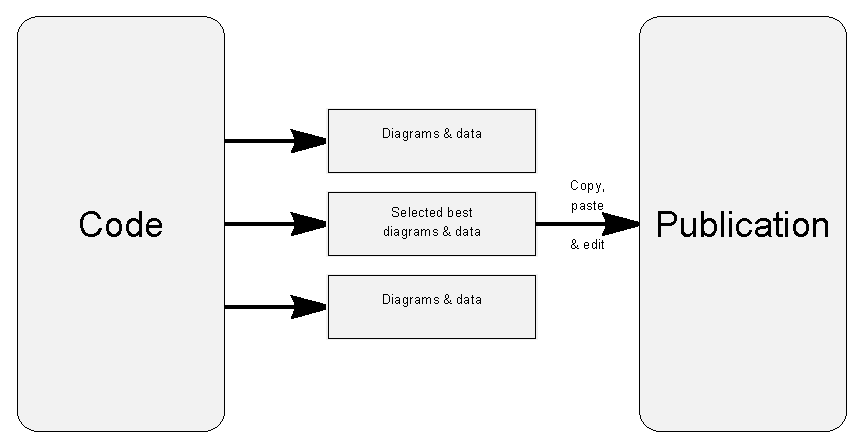
\includegraphics[width=5in]{generated/basic.pdf} 
   \caption{The common basic --- error-prone and obsolete --- approach to scientific authoring is to use code to help generate analyses and diagrams, then manually copy and paste the selected results into the publication. Note that the publication, including the results, can be edited arbitrarily, and typically the results published will have been edited and modified (if only for typographical purposes) from those actually generated by the code.}
   \label{fig:basic}
\end{figure}
\begin{figure} 
   \centering
   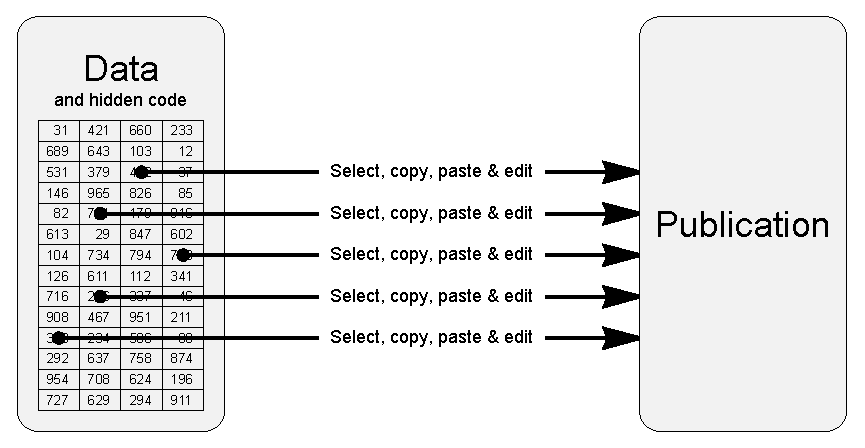
\includegraphics[width=5in]{generated/excel.pdf} 
   \caption{When the code is in a spreadsheet, such as Microsoft Excel, the code is generally hidden from sight. The data copied \& pasted into a publication may or may not be calculated from data in other cells (such as column totals). Records are rarely taken of these manual processes, and, anyway, typically it is impossible to be certain exactly what has been copied unless very great care is taken. In consequence, if a spreadsheet is modified, it is haphazard what results are updated and corrected in the publication. }
   \globalLabelValue{excelFigure}{\thefigure}
   \label{fig:excel}
\end{figure}
\begin{figure} 
   \centering
   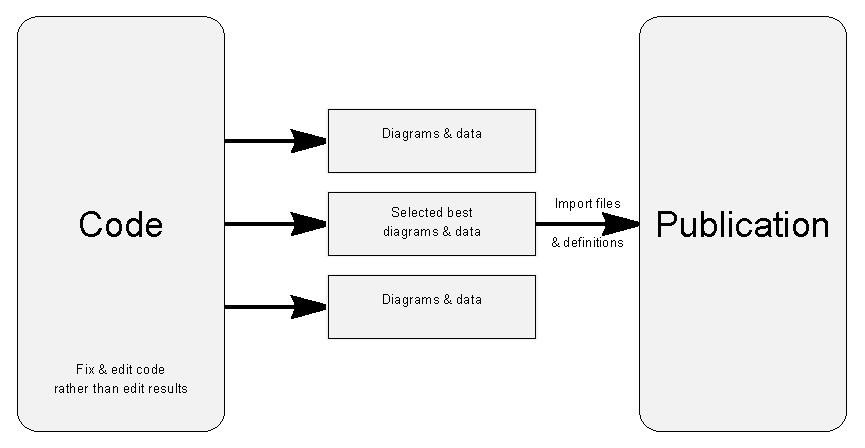
\includegraphics[width=5in]{generated/import.pdf} 
   \caption{Improving over the normal approach (figure \ref{fig:basic}), data and diagrams are placed in the publication using a programmed, systematic approach. In the present paper, this was done by generating text files of \LaTeX\ definitions (represented by boxes in the central column of the schematic), hence providing \LaTeX\ names for all of the code-generated values. Since the copying of results into a publication is automated and easy, any improvements to the results (such as correcting errors) are made by improving the code --- which therefore contributes to improving all future-generated results too. Not shown, but in well-engineered code, documentation will also be generated, such as by using tools such as JavaDoc or Doxygen.}
   \label{fig:rap}
\end{figure}
\begin{figure}[t]
   \centering
   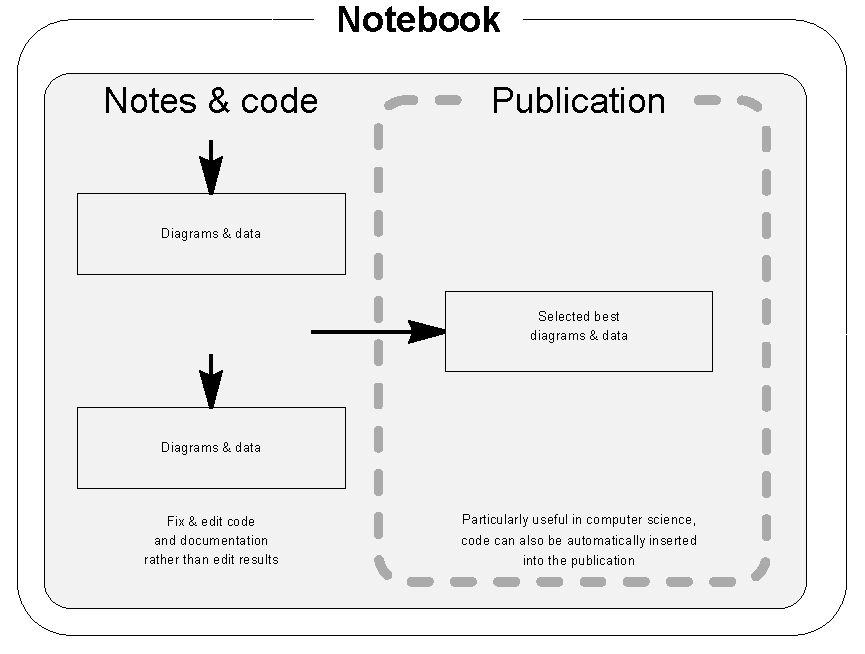
\includegraphics[width=5in]{generated/notebook.pdf} 
   \caption{In a notebook system, such as \emph{Mathematica\/} or Jupyter, a single document --- the notebook --- integrates the publication, the code, any notes, as well as all the results. The code generates results and images that are automatically (and reliably) inserted in place into the notebook, usually right after the code that generates them. Some parts of the notebook are marked or selected to be printed as the publication, thus allowing most if not all code to be hidden from the final publication. In well-engineered code, the notebook will directly contain full documentation.
Note that in most systems, notebooks can import and generate arbitrary data (images, sounds, sensor data, etc).}
   \label{fig:notebook}
\end{figure}

\changemysection{The Spiegelhalter trustworthiness questions}
\globalLabel{supplementary-Spiegelhalter-section}

David Spiegelhalter is concerned how statistics is often misused and misunderstood. In his \emph{The Art of Statistics\/} \cite{Spiegelhalter} Spiegelhalter brings together his advice for making reliable statistical claims: they need to be accessible, intelligible, assessable, and usable --- and the claims need to be properly accountable. 

Spiegelhalter proposes ten questions to ask when confronted with any claim based on statistical evidence. Some of his questions are quite general, and might be applied to any sort of scientific claims, but all have analogous questions that could be addressed to software code or publications relying on code --- analogues are suggested in \textbf{bold} below. 

What might seem like dauntingly technical software issues are no more demanding than the basic statistical issues that are regularly acceded to; failing to ask these questions is as risky as dismissing statistical scrutiny.

\def\questionsection#1{\changemysubsection{#1}}
\def\question#1{\item \emph{#1\/}}
\def\sequestion#1{\begin{itemize}\raggedright\item[$\blacktriangleright$] \textbf{#1}\end{itemize}}

\questionsection{How trustworthy are the numbers?}
\newcounter{resumeCounter}

\begin{enumerate}
\question{How rigorously has the study been done?} For example, check for `internal validity,' appropriate design and wording of questions, pre-registration of the protocol, take a representative sample, using randomization, and making a fair comparison with a control group.

\sequestion{How rigorously has the Software Engineering been done? Section \ref{supplementary-best-practice} in the \supplement\ provides a list of important issues that must be addressed for any reliable software.}

\sequestion{``Internal validity'' assumes that there is evidence the programmers had uncertainty in the code's reliability and checked it. Were different methods used and compared, or was all confidence put into a single implementation? What internal consistency checks does the implementation have? Were invariants and assertions defined and checked? }

\question{What is the statistical uncertainty/confidence in the findings?} Check margins of error, confidence intervals, statistical significance, multiple comparisons, systemic bias.

\sequestion{How are the claims presented that give us confidence in the code that they are based on? Are there discussions of invariants, independent checks for errors, and so on? Again, \supplement\ section \ref{supplementary-best-practice} provides further discussion of such issues.}

\question{Is the summary appropriate?} Check appropriate use of averages, variability, relative and absolute risks.

\sequestion{If the claims are exploratory, weaker standards of coding can be used; if the claims are a basis for critical decisions, then there should be evidence of using appropriate Software Engineering (such as defensive programming) to provide appropriate confidence in the results claimed.}
\setcounter{resumeCounter}{\value{enumi}}
\end{enumerate}
\questionsection{How trustworthy is the source?}
\begin{enumerate}
\setcounter{enumi}{\value{resumeCounter}}
\question{How reliable is the source of the story?} Consider the possibility of a biased source with conflicts of interest, and check publication is independently peer-reviewed. Ask yourself, `Why does this source want me to hear this story?'

\sequestion{The source of many science stories is the output of running some code. How reliable is this code? What evidence is there that the code was well-engineered so its reliability can be trusted?}

\sequestion{What evidence is there of rigorous (e.g., code review and tool-based) independent methods being used to manage coding bias?}

\question{Is the story being spun?} Be aware of the use of framing, emotional appeal through quoting anecdotes about extreme cases, misleading graphs, exaggerated headlines, big-sounding numbers.

\sequestion{Be wary of AI and ML which may have been trained by chance or specifically (if not deliberately) to get the results described.}

\question{What am I not being told?} This is perhaps the most important question of all. Think about cherry-picked results, missing information that would conflict with the story, and lack of independent comment.

\sequestion{Cherry picking with code is often unconscious and is very common: when running code produces the ``cherries'' for a paper it is tempting to stop testing the code, and just assume it is running correctly. So, what evidence is there that the code was rigorously developed and cherry picking avoided?}

\setcounter{resumeCounter}{\value{enumi}}
\end{enumerate}
\questionsection{How trustworthy is the interpretation?}
\begin{enumerate}
\setcounter{enumi}{\value{resumeCounter}}
\question{How does the claim fit with what else is known?} Consider the context, appropriate comparators, including historical data, and what other studies have shown, ideally in a meta-analysis.

\sequestion{Is there any discussion of the code and how does it compare with other peer-reviewed publications using code used for similar purposes?}

\question{What's the claimed explanation for what has been seen?} Vital issues are correlation v.\ causation, regression to the mean, inappropriate claim that a non-significant result means `no effect,' confounding attribution, prosecutor's fallacy.

\sequestion{These are all good statistical questions. The Software Engineering analogy is: are the claims backed up by a sufficiently detailed discussion of the algorithms and Software Engineering that justify the appropriateness of the chosen software implementation? The \supplement\ list in section \ref{supplementary-best-practice} provides examples of expected explanations for the trustworthiness of running some code.}

\question{How relevant to the story is the audience?} Think about generalizability, whether the people being studied are special case, has there been an extrapolation from mice to people.

\sequestion{Generalizability is equivalent to is the code available, easy to understand and use for more general purposes --- including further work and checking the reproducibility of the claims being made?}

\question{Is the claimed effect important?} Check whether the magnitude of the effect is practically significant, and be especially wary of claims of `increased risk.'
\end{enumerate}

\newcount\temporary \temporary=\mainNumberOfReferences
\newcount\temporaryPlusOne \temporaryPlusOne=\temporary
\advance \temporaryPlusOne by 1
\def\MaxMainPaperCitationNumber{\the\temporary}

\highlightmysection{A pilot survey of computational science}
\globalLabel{survey-section}

The main paper was motivated by selected epidemiological papers and their problematic computational models (which are discussed in the paper). Are the issues illustrated by these case studies typical of science more broadly? We undertook, then, some selected studies of papers in different fields, then undertook a randomized, stratified pilot survey covering several leading peer reviewed journals. The point was not to establish the frequency of problems, so much as to sign whether the problematic case study was exceptional or typical. 

%There are many ways to do good science. Normal science routinely involves either performing new research and reporting it in the literature, or performing reviews --- such as systematic reviews --- of the existing literature to form a consensus view of an existing body of research. Typically, research offers new theories or results, points out previous errors, or uses statistical or qualitative methods to reduce the variability in previously reported results. In any case, the intention is to provide reliable knowledge and to bolster consensus \cite{ziman}.

%In the present case, we have identified limitations in the methodology of certain scientific contributions, throwing doubt on their soundness and reliability; furthermore, we identified critical misunderstandings in the literature citing those papers, including misunderstanding the nature of code reproducibility. 

%It is possible, if not likely (e.g., given the report in \emph{Nature\/}, cited above \cite{nature-review}), that such limitations are more widespread than the specific examples considered so far, which are anyway limited primarily to epidemiology, and to COVID research performed under extreme pandemic pressure. We now therefore undertake a small, manageable stratified sample of peer reviewed literature to explore whether the issues are more widespread.

The pilot study follows the RAP methodology. The data and code for this paper's pilot survey (and all other analysis used in the paper and in this \supplement) are available on GitHub. All raw data is converted into \LaTeX\ so that the analysis can be typeset directly in the paper; this \supplement\ also contains a complete tabular presentation of the data.

Moreover, this paper itself follows the more general \RAPstar\ methodology. For example, as standard practice, a Unix makefile is used to make it easy to analyze and generate all data, typeset the paper, and more. Table \ref{table:options} shows the options provided.

\begin{table}[t]
\begin{center}
\input generated/make-help.tex
\end{center}
\caption{Conforming to the \RAPstar\ methodology, the abbreviated summary above was generated automatically, by using \texttt{make data}. %(Saying \texttt{make help} would generate a full summary on the command line.)
}
\label{table:options}
\end{table}

The \RAPstar\ approach cannot enforce the truth of such as summary, but it very significantly increases the chances that the summary is correct and up to date. For example, if refactoring leads to an option being deleted, then it will also disappear \emph{with no further work\/} from the table above. Also, since the summary was proof-read at the same time as proof-reading this \supplement, following \RAPstar\ also increases the chances that any errors or functionality omissions or issues in the makefile have been detected and corrected.

\highlightmysubsection{Selected journal case studies}

The journal \emph{The Lancet\/} published and then subsequently retracted a paper on using hydroxychloroquine as a treatment for COVID \cite{lancet-retracted}. The paper was found to rely on fraudulent data \cite{science-lancet1,science-lancet2}. \emph{The Lancet\/} subsequently tightened its data policies \cite{lancet-learning}, for instance to require that more than one author must have directly accessed and verified the data reported in the manuscript. Curiously, the original (now retracted) paper declares 
\begin{quote}\sf
\setbox0=\hbox{``}\hskip -\wd0\copy0 \ldots\ all authors participated in critical revision of the manuscript for important intellectual content. MRM and ANP supervised the study. All authors approved the final manuscript and were responsible for the decision to submit for publication.'' \end{quote} 

which seems to suggest that several original authors of the paper would have been happy to make the new declarations --- and, of course, if there is fraud (as was established in this case) it seems likely that authors who make the new declarations of accessing and verifying data are unlikely to make reliable declarations. 

\emph{The Lancet\/} still has no code publication policy, and for more than one author to have ``direct access'' to the data they are very likely to access the data through the same code. If the code is faulty or fraudulent, an additional author's confirmation of the data is insufficient, and there is at least as much reason for code to be fraudulent (not least because code is much harder to scrutinize than data). Code needs more than one author to check it, and ideally reviewers independent of the authors so they do not share the same assumptions and systems (for instance shared libraries, let alone potential collusion in fraud).

In 2020 the \emph{Journal of Vascular Surgery\/} published a research paper \cite{jvs1}, which had to be retracted on ethical grounds \cite{jvs2,jvs3}: it was a na\"\i ve study and the editorial process was unaware of digital norms. Notably, the paper fails to provide access to its anonymized data (with or without qualification), and fails to define the data anonymization algorithm, and also fails to even mention the code that it developed and used to perform its study. The journal's data policy is itself very weak (the authors ``should consider'' including a footnote to offer limited access to the data) and, despite basic statistics policies, it has no policy at all for code (see  section \ref{supplementary-journal-policies-section}). Ironically, the retracted article \cite{jvs1} is still online (as of August 2020) with no reference to any editorial statement to the effect that it has been retracted, despite this being trivial --- and necessary --- to achieve in the widely-accessed online medium.

Medical research often aims to establish a formula to define a clinical parameter (such as body mass index, BMI) or to specify an optimal drug dose or other intervention for treatment. These formulas, for which there is conventional clinical evidence, are often used as the basis for computer code that provides advice or even directly controls interventions. Unfortunately a simple formula as may be published in a medical paper is \emph{never\/} sufficient to specify code to implement it safely. For example, clinical papers do not need to evaluate or manage user error when operating apps, and therefore the statistical results of the research will be idealistic compared to the outcomes using an app under real conditions --- which is what the clinical research is supposedly for. A widespread bug (and its fix) that is often overlooked is discussed in \cite{numerals}; the paper includes an example of a popular clinical calculator (based on published clinical research) that calculated nonsense, and potentially dangerous, results. The paper \cite{fda} summarizes evidence that such bugs, ignored by the clinical research literature, are commonplace in medical systems and devices.

\highlightmysubsection{Pilot paper sample}
A sample of \plural{\dataN}{recent paper} covering a broad range of science were sampled from the leading journals \journalBreakdown. 

\makeatletter
\long\def\@makecaption#1#2{%
  \vskip\abovecaptionskip
  \sbox\@tempboxa{#1: #2}%
  \ifdim \wd\@tempboxa >\hsize
    \textbf{#1}: #2\par
  \else
    \global \@minipagefalse
    \hb@xt@\hsize{\hfil\box\@tempboxa\hfil}%
  \fi
  \vskip\belowcaptionskip}
\makeatother

\begin{table*}[t]
\begin{center}
\begin{tabular}{|rl|} \hline
\the\numberOfJournals&Journals\\
\the\dataN&Papers:\\
\tabularJournalBreakdown
\the\countAuthors&Published authors\\
\the\totalPages&Published journal pages\\
July 2020&Sample month\\ \hline
\end{tabular}
\end{center}

%\newcount \total
%\total=\dataN
%\multiply \total by 4 % three reviewers, one editor
%\advance \total by \countAuthors
%\the\total\
%leading scientists assuming authors, 1 editor, and 3 reviewers per paper, but not counting acknowledged colleagues et al, covering  (plus appendices and supporting material) in total.
%
\caption{Overview of the peer-reviewed paper sample.}
\label{supplement-table-overview}
\end{table*}

\begin{table*}[t]
\begin{center}\normalsize
\input generated/summary-table.tex
\end{center}

\caption{Summary of survey results.}
\label{supplement-table-summary}
\end{table*}

\begin{table*}[t]

\def\reponame#1#2{{\tt #1} \csname cite-#2\endcsname}

\expandafter\def\csname pagelength-covid-sim\endcsname{20}
\expandafter\def\csname cite-covid-sim\endcsname{\cite{ICmodel}}

% divide #1 by #2
\newcount \uu
\newcount \vv
\newcount \ww
\def\makeAverage#1#2{%
	\uu=#1
	\vv=#2
	\multiply \uu by 1000
	\divide \uu by \vv
	% uu is now 1000 times the answer we want
	\ww = \uu
	\divide \uu by 1000
	\multiply \uu by 1000
	\advance \ww by -\uu
	\divide \uu by 1000
	%[ #1 / #2 = \the\uu .\the\ww\ ]
	\ifnum \ww > 499 \advance \uu by 1 \fi
	\the\uu
}

\begin{center}

\expandafter \advance \gitPages by \csname pagelength-covid-sim\endcsname

\input generated/repos.tex
\vskip 1ex
\small Citation numbers $>$ \MaxMainPaperCitationNumber\ can be found in the \supplement
\\
\small Repository clones downloaded and automatically summarized \clonedate
\end{center}

\caption{Sizes of repositories, with approximate sizes of code (in kLOC) and data for all available GitHub repositories reviewed in the survey, plus \texttt{covid-sim} \cite{ICmodel} for comparison. Sizes are approximate because in all repositories code and data are conceptually interchangeable (an issue explained in the \supplement), so choices were made in the survey to avoid double-counting. Many repositories rely on downloading additional code and data, which is not counted in the table as the additional required material is not in the repository cited in the paper.  At the time of cloning and checking all repositories in \clonewhen, paper \csname cite-PostoperativeOutcomes.RiskNet\endcsname\ still had nothing in its repository except a single file still saying ``...code coming soon...,'' despite \the\pubdelayinmonths\ months having already elapsed since the submitted paper had claimed the code could be accessed in its repository.}
\label{table-repo-summary}\globalTableLabel{supplementaryTableRepoSummary}
\end{table*}

The two journals \emph{Nature Digital Medicine\/} and \emph{Lancet Digital Health\/} were selected as leading specialist science journals in an area where correctness of scientific modeling has safety-critical implications, and \emph{Royal Society Open Science\/} was selected as a leading general science journal. All papers sampled are Open Access, although for some papers some or all of the associated data has no or restricted access, in some cases despite the relevant journal policies on code. Table \ref{supplement-table-overview} is an overview of the sample.  

Papers were selected from the journals' July 2020 then new online listings where the paper's title implied that code had been used in the research. Commentary, correspondence, and editorials were excluded. The sample is intended to be large enough and objective enough to avoid the selection bias in the papers that motivated the current paper (the sample excludes the motivating papers discussed above as they were not published in the sampled journals), so that the sample may be considered to fairly represent what the editorial and the broader peer review community in leading journals considers to be good practice for computationally-based science. The selection criterion selected papers where the title implies the authors themselves considered code to be a significant component of the scientific contribution, and, indeed, all sampled papers relied on and assumed the quality of code used in their research. 


This convenience sample may be considered to be small given the importance of the research questions and relative to the diversity and huge number of scientific papers,\footnote{Using Google Scholar it is estimated that over 40,000 papers meeting the title criteria were published in the month of July 2020.} but~\ldots

\begin{enumerate}
\item the selected journals are leading peer-reviewed scientific journals that set the standards for scientific publishing practice generally (although the sample shows that code policies are not always enforced); 

\item as will be clear from the following discussion, there is little variation across the sample, which implies that a larger sample would not have been productively more insightful (this view is consistent with the multi-disciplinary reports in \cite{nature-review}, mentioned in section \ref{section-science-beyond-pandemic-modeling}); 

\item the survey is not intended to be a formal, systematic sample of scientific research in general, but is intended to be sufficient to dispel the possibility that the issues described above earlier in this paper are isolated practice unique to a few papers in epidemiology, perhaps an idiosyncrasy of a few authors in a particular field, or perhaps due to an initial chance selection bias (e.g., the Ferguson papers were reviewed above because of Ferguson's public profile and the importance of dependable pandemic research, but they might have just happened to be Software Engineering outliers);

\item the code/data policies of the \plural{\numberOfJournals}{journal} condoned at the time of the sample \emph{and continue to condone\/} poor practice at the time of writing the present paper (\monthname{\month} \the\year) --- for specific details and further explanation of the problems, see \supplement\ section \ref{supplementary-journal-policies-section};

\item
the fact that the specifically identified problems are elementary errors in Software Engineering (see the discussion in section \ref{section-discussion}) suggests more sophisticated analysis is not required;

\item 
finally, the present paper's \LaTeX\ source, as well as all documented code and data, are available from a repository, which provides a convenient framework for easily refining or developing the research as may be desired (see details at the end of this paper).
\end{enumerate}

The \the\dataN\ papers surveyed cover a range of specialities, and it is unlikely that non-specialists can properly assess the code from the point of view of the specialism, not least because many of the papers sampled require specialist code libraries (and in the right combinations of versions) to be run that not everyone will have or be able to install. Code quality was therefore assessed by reading it --- due to the paper authors' complex and/or narrative interpretation of data, code, data and hardware/operating system dependencies, no assessment could realistically be made whether the code provided actually reproduced a paper's specific claims. Indeed, if we trust the papers that their code was actually run and provides the results as reported, then running their code (when provided in full) would merely check the paper/code consistency but will not assess the quality or reliability of the code. Indeed, in most scientific papers there are layers of expert scientific work, interpretation and abstraction, lying between the computational models and the report in the paper.

\highlightmysubsection{Summary of results}
\label{summary-of-results}
The sample selection criteria necessarily identified scientific research with Software Engineering contributions. 

No evidence of verification and validation was seen. There was only one example of very basic Software Engineering methods, namely independent coding, and even then the independent code used for testing was not uploaded to the paper's code repository, so the independent testing is not available for reviewers or readers of the paper. (See \supplement\ for more details.)

There was no evidence of any critical assessment of code, suggesting that scientists writing papers take it for granted that their code works as they intend. No competent programmer would take it for granted that their code was correct without following rigorous methods, such as formal methods, regression testing, test driven design, etc. (See the \supplement\ for a list of standard methods.)

Much code depended on specific software versions, specific libraries, and substantial manual intervention to compile it. All code (where actually provided) was sufficiently complex that, if it was to be used or scrutinized, required more substantial documentation than was provided.

On the whole, on the basis of the sample evidence, scientists do not make their code \emph{usably\/} available, and rarely provide adequate documentation (see table \ref{supplement-table-summary}). 

With the one minor exception, no papers reported anything on any Software Engineering methodologies, which is astonishing given the scale of some of the software effort supporting the papers (table \ref{table-repo-summary}).  The papers themselves, typically only a few published pages, are very brief compared to the substantial code they rely on (see table \ref{table-repo-summary}). 

With the one exception, none of the papers used any specific Software Engineering methods, such as open source \cite{open-source} or other standard methodologies provided in this \supplement, to help manage their processes and help improve quality. Although software stability \cite{stability} is a relatively new concept, understood as methodologies, such as portability, to provide long-term value of software, it is curious that none of the papers made any attempt at stability (however understood) despite the irony that all the papers were published in archival journals.\footnote{Reasons the present paper does not directly assess the quality of software in the surveyed papers include: many papers did not provide complete software; it was not possible to find correct versions of all software systems to run the models; also, no papers provided adequate test suites so that correct operation of software could be confirmed objectively.}

\emph{Nature Digital Medicine\/} and \emph{Royal Society Open Science\/} have clear data and code policies (see \supplement\ section \ref{supplementary-journal-policies-section}), but actual publishing practice falls short: \the\countHasBreach\ out of the \plural{\countHasPolicy}{paper} (\pc{\countHasBreach}{\countHasPolicy}) published in them and sampled in the survey manifestly breach their code policies. In contrast, \emph{Lancet Digital Health\/}, despite substantial data policies, has no code policy at all to breach. The implication is that the fields, and the editorial expertise of leading journals, misunderstand and dismiss code policies --- they (or their editors and reviewers) are technically unable to assess them. This lack of expertise is consistent with the limited awareness of Software Engineering best practice that is manifest in the published papers (and resources) themselves.

Code repositories were used by \plural{\countUsesVersionControlRepository}{paper} (\pc{\countUsesVersionControlRepository}{\dataN}), though \plural{\countNoCodeInRepo}{paper} in the survey claimed to have code on GitHub but there was no code in the repository, only the comment ``Code coming soon\ldots'' (checked at the time of doing the review, then double-checked as detailed in the references in the \supplement, as well as most recently on \clonedate\
while checking table \ref{table-repo-summary}): in other words, the repository had never been used and the code could never have been looked at, let alone reviewed.\footnote{GitHub records show that it had not been deleted after paper submission.} This is a pity because GitHub provides help and targeted warnings and hints like ``No description, website, or topics provided [\ldots] no releases published.'' The lack of code is ironic: the paper concerned \csname cite-PostoperativeOutcomes.RiskNet\endcsname\ has as its title ``\emph{Development and validation\/} of a deep neural network model [\ldots]'' (our emphasis), yet it provides no code or development processes for the runnable model it claims to validate, so nobody else (including referees) can check any of the paper's specific claims.

The sizes of all GitHub repositories are summarized in table \ref{table-repo-summary} (since many papers not using GitHub do not have all code available, non-GitHub code sizes are not easily compared and are not listed). 

Overall, there was no evidence that any code had been developed carefully, let alone by using recognized professional Software Engineering methods. In particular, 
\ifnum \countCodetested=0
no papers
\else only \plural{\countCodetested}{paper}
\fi in the survey provide any claims or evidence of effective testing, for instance with evidence that tests were run on clean builds. {While it may sound unrealistic to ask for evidence on software quality in a paper written for another field of science, the need is no less than the need for standard levels of rigor in statistics reporting, as discussed in the opening of this paper.}

Data repositories (the Dryad Digital Repository, Figshare or similar) were used by \plural{\counthasDataRepository}{paper} to provide structured access to their data. Unlike GitHub, which is a general purpose repository, Dryad has scientifically-informed guidelines on handling data, and all papers that used Dryad provided more than just their raw data --- they provided a little, sometimes substantial, documentation for their data. At the time of writing, Dryad is not helpful for managing code --- its model appears to be founded on the requirement that once published papers must refer to exactly the data they used, so further refinements on the data (or code) are taboo, even with version control.

\highlightmysubsection{Current code policies of sampled journals}
\globalLabel{supplementary-journal-policies-section}

It is noteworthy that none of the journals sampled permit any reliable style of managing data in published papers, such as described above in sections \ref{detecting-against-error} and \ref{restrictive-policies}. In particular, for all the papers that had accessible code, the code included explicit (and relevant) data that was not archived \emph{as\/} data in the journal repositories.

Note that journal policies were first accessed on 29 July 2020, close after the period covered by the pilot survey, thus presumably fairly closely reflecting the policies in use for the papers in the survey on the dates when they were each submitted. Unfortunately for the survey, the journals do not make clear what exact policies were applied to each paper when the papers were submitted (on the other hand, the survey shows that policies are not rigorously enforced).
\\

\newdimen\tabwidth
\tabwidth=\textwidth
\advance \tabwidth by -4em
\def\specifyurl{\vskip 3mm
\begingroup\raggedleft\scriptsize
} 
\def\specifyurletc#1{\endgroup\\
\hbox{ }\hfill\begin{tabular}{|p{\tabwidth}@{}}
#1
\end{tabular}\vskip .3cm
}

{\sf
\noindent\textbf{Extract from \emph{Royal Society Open Science\/} author guidelines} \\
--- It is a condition of publication that authors make the primary data, materials (such as statistical tools, protocols, software) and code publicly available. These must be provided at the point of submission for our Editors and reviewers for peer-review, and then made publicly available at acceptance. [\ldots] As a minimum, sufficient information and data are required to allow others to replicate all study findings reported in the article. Data and code should be deposited in a form that will allow maximum reuse. As part of our open data policy, we ask that data and code are hosted in a public, recognized repository, with an open licence (CC0 or CC-BY) clearly visible on the landing page of your dataset.}

\specifyurl
\url{royalsociety.org/journals/authors/author-guidelines/#data}
\specifyurletc{Since first accessed 29 July 2020, the policy has been revised (undated, accessed 2 February 2022) but retains the same principles; full policy now available via a DOI \cite{RS-policy}. The policy still retains an emphasis on data accessibility, and continues a lack of awareness that code and data are equivalent and often mixed (see section \ref{on-code-data-publication}).}

\noindent\textbf{Extract from \emph{Nature Digital Medicine\/} author guidelines}\\
{\sf --- A condition of publication in a Nature Research journal is that authors are required to make materials, data, code, and associated protocols promptly available to readers without undue qualifications. [\ldots] A condition of publication in a Nature Research journal is that authors are required to make unique materials promptly available to others without undue qualifications.}

\specifyurl
\url{www.nature.com/nature-research/editorial-policies/reporting-standards#availability-of-data}
\specifyurletc{Accessed 29 July 2020; since updated (accessed 2 February 2022) to require [in part] ``Upon publication, Nature Portfolio journals consider it best practice to release custom computer code in a way that allows readers to repeat the published results. Code should be deposited in a DOI-minting repository such as Zenodo, Gigantum or Code Ocean and cited in the reference list following the guidelines described here.'' 
}

\noindent\textbf{\emph{Lancet Digital Health\/} author guidelines}\\
Journal has detailed data policies, but no code policy.

\specifyurl
\url{marlin-prod.literatumonline.com/pb-assets/Lancet/authors/tldh-info-for-authors.pdf}
\specifyurletc{Accessed 29 July 2020. Still no code policy when accessed 2 February 2022.}

\noindent\textbf{Extract from \emph{Journal of Vascular Surgery\/} author guidelines}\\
The \emph{Journal of Vascular Surgery\/} has detailed data policies, but no code policy. While no \emph{Journal of Vascular Surgery\/} papers were surveyed, the following statement on data policies is relevant:

\vskip 3mm \noindent {\sf --- The authors are required to produce the data on which the manuscript is based for examination by the Editors or their assignees, should they request it. [\ldots] The authors should consider including a footnote in the manuscript indicating their willingness to make the original data available to other investigators through electronic media to permit alternative analysis and/or inclusion in a meta-analysis.}
\specifyurl
\url{www.editorialmanager.com/jvs/account/JVS_Instructions%20for%20Authors2020.pdf}
\specifyurletc{Accessed 29 July 2020. Policy unchanged when accessed 2 February 2022.}

\label{data-methods-section}
\highlightmysubsection{Assessment criteria and methods}
\label{data-methods-subsection}
A survey sampled of recent papers that were published online in July 2020, accepted for publication after peer review in \the\numberOfJournals\ high-profile, highly competitive leading peer-reviewed journals, namely \journalBreakdown. Papers were selected from the journals' July 2020 new online listings where the paper's title implied that code had been used in the research. Commentary, correspondence and editorials were excluded. The sample represents what the editorial and the broader peer review community considers to be good practice. 

The selection process will have certainly missed some papers that use code, but the criterion selects papers where the wording of the title indicates that the authors consider code to be a component of the scientific contribution. Indeed, all sampled papers used code in their research. Although there is unavoidable subjectivity in the paper evaluations and uncontrolled bias from using a single evaluator (the author of this paper), it is hoped that using a sample of \plural{\dataN}{paper} from \plural{\numberOfJournals}{diverse journal} is sufficient to randomize errors so that they largely cancel out, and the overall trends as discussed in this paper are reliable. It should be noted that, except where a paper provides a URL to a code repository, much code was disorganized so possibly not all code was reviewed because it was too hard to find (some emails to authors have not been responded to). 
 
Since almost every scientific paper relies on generic computer code (calculating statistics, plotting graphs, storing and manipulating data, accessing internet resources, etc), the baseline of papers using code was not assessed. Papers whose title indicated their contribution included or relied on bespoke code were selected, and all those clearly relied heavily on their own specifically developed code. Papers that may have relied on bespoke code but whose titles made no such implication were not assessed.

Although the pilot survey is not a systematic review, following Preferred Reporting Items for Systematic Reviews and Meta-Analyses (PRISMA) \cite{prisma} it is good practice to disclose details of the reviewers. In the present case, the selected papers were assessed by the author of the present paper. The study was not blinded. This is, of course, a limitation of the study. However, the reviewer is a full professor of computer science, who has taught and assessed computer software since the 1970s, using moderated and peer-reviewed processes for undergraduate and postgraduate computing degrees, and is well aware assessing code quality has been a lively topic in Software Engineering for decades (there is now international standard ISO/IEC 9126, updated to ISO 25000). The author has written legal documents analyzing software for criminal cases involving faulty software. The author has approximately 
\newcount \papers \papers=340 % peer reviewed
\advance \papers by 188 %invited
\the\papers\ published papers in computer science. 

The evaluations performed for the present paper are at a trivial level where sources of bias should have a negligible effect, particularly given that the overall conclusion is consistent across both the diverse sample and the computational science-based papers cited in the paper that did not form part of the selected sample. As said in the body the paper: \emph{the fact that the specifically identified problems are elementary errors in Software Engineering (see the discussion in \emph{[main paper]\/} section \ref{section-discussion}) suggests more sophisticated analysis is not required}. 

In any case, as stated in the main paper, the full dataset and analysis code is available at \begin{center}\url{github.com/haroldthimbleby/Software-Enginering-Boards}\end{center} and the reviewed papers are (unless retracted) still available online for independent assessment. %The data is also provided in full later in this \supplement.

There is considerable debate over what good commenting practice is, but this is because comments have many roles --- from helping students to get marks in assessments, asserting intellectual rights, reminding the developer of things to do, managing version control, to explaining the code to third parties. Different programming languages also develop ``cultures'' and tool-based systems that encourage different approaches for comments (examples include R Markdown, Mathematica Notebooks, JavaDoc, Haskell's Haddock, and so on). For scientific code, however, the explanatory role is critical, and this is what was assessed in the present survey. It is notable that no such tool-based approach to code or documentation was used in any code reviewed.

The completeness or executability of code was not assessed, although if code was obviously incomplete this was noted. Whether code runs as claimed is a matter of research integrity, which is beyond the scope of this survey. What is relevant to the study is whether the code is described in sufficient detail that the methods used can be scrutinized. Obviously being able to run the code will help, but clarity in documentation and comments is critical. It is more like ``can we see the critical pages from your lab book so we understand what you did?''\ rather than ``can we have a free run of your laboratory, even though we don't understand the details of the science?''

As an informal survey, intended to establish whether the issues in epidemic modeling were more widespread, and given the very poor level of documentation found in scientific code, it was not felt necessary to have independent or blind assessment.

The data was recorded in JSON (JavaScript Object Notation), which is a simple standard data format. A typical entry in the data file looks like this (with long field values truncated for clarity):

\newdimen \codeIndent
\codeIndent = 1em
\vskip 1ex
\vbox{%
  \input generated/example-data.tex
}
\vskip 1ex

The data was entered by hand (as JSON terms), after reading and reviewing each paper in the survey. In total there are \the\countFields\ data fields available for documenting papers, but not all need be used for each paper; for example, the field \texttt{hasCodeTested} defaults to \texttt{false}, so it need not be set --- it is also an error to set it if another field asserts there is no code to evaluate! (A separate JSON data structure maps the data fields to English descriptions, along with default values if they are optional descriptors.)

A JavaScript program sanity checks the JSON data. The sanity checks found a few errors (e.g., it checks that if there are comments of any sort then there must be some accessible code; it checks the DOI is accessible, etc), which led to a productive double-checking of all the facts of the original papers --- and correcting all the errors. Some papers that had had no code available during the first assessment had uploaded code by the time of the double-checking.\footnote{{Note that double-checking was performed by the same person as the first assessment, though with the benefit of a six month gap to bring a degree of independence}.} A field \texttt{doubleChecked} was added to supplement the original data field \texttt{accessed} to track the process of double-checking the data; the sanity checks then of course checked all \texttt{doubleChecked} fields were completed.

Note that since JSON data is JavaScript code, it was convenient to combine the data, the data sanity checking, and the analysis all in a single file. Hence, running the data generates the core human-readable information used in this paper.

The JavaScript data+program generates files from the JSON; these files were then included in both the main paper and in this \supplement, so when the paper or \supplement\ is typeset all tables and specific data items are typeset automatically, consistently and reliably by \LaTeX\@.

For example, the register \texttt{\bslash dataN} is set to the value \the\dataN, which is the total number of papers assessed in the JSON data, and the macro \texttt{\bslash journalBreakdown} is defined directly from the data to be the following text (when typeset in \LaTeX):

\begin{quote}
\journalBreakdown 
\end{quote}

--- which is the breakdown of the total $N=\the\dataN$ by journal name. The \emph{exact\/} same text was also used in the main paper. 

An interesting consequence of this automatic approach is that as the author found themselves starting to write text such as:

\begin{quote}
\tt Code repositories were used by \plural{\countUsesVersionControlRepository}{paper} \ldots
\end{quote}

it motivated extending the JavaScript data processing so that \emph{all\/} specific quantities mentioned in the paper are traceable directly back to the JSON data. The phrase above is now in fact written in \LaTeX\ in the paper as follows:

\begin{quote}\tt\small
Code repositories were used by \\
\bslash plural\{\bslash countUsesVersionControlRepository\}\{paper\} \ldots
\end{quote}

where {\tt\small \bslash plural} automatically writes a word (``paper'' in this case) in singular or plural form as required. 

Each of the \plural{\dataVariableCount}{variable} used in the paper were defined in automatically-written \LaTeX\ header files that declare them and assigns appropriate values. The header files are included in the paper using \LaTeX's standard \texttt{\textbackslash input} command. Here is an example of one such automatic definition:

\begin{verse}\tt
\textbackslash newcount \textbackslash dataVariableCount \\
\textbackslash dataVariableCount = \the\dataVariableCount
\end{verse}

so the named value is then available for the author to use when the paper is typeset.

Some of the files generated from the JSON data are Unix shell scripts. For example, details of all the papers with GitHub repositories are automatically collected into a shell script so the repositories can be cloned locally and then measured (as it happens, using \texttt{awk} scripts), e.g., to generate table \ref{table-repo-summary} for this \supplement.

The full JavaScript JSON data and processing code (including the makefile) is provided in this paper's repository, as described in the main paper.

% This commented-out sentiment is repeated later...
% Finally, because of their approach to automatic typesetting, some journals require that no files are explicitly \texttt{input} into \LaTeX, so a simple program is provided in the GitHub repository to recursively expand all \texttt{input} commands before submission. If the source files are available for download after this paper is accepted, they will therefore contain no \texttt{input} commands, but they will contain comments at the appropriate points in the expanded source code explaining the sources of the \texttt{input} data. It is curious that the journals cannot do this for themselves.

\highlightmysubsection{Detecting and defending against error}
\label{detecting-against-error}
% check it works for other numbers 
%\countUsesVersionControlRepository=296

Normally, when we write a number like \the\countUsesVersionControlRepository\ in a paper, especially longer or more complex numbers, we will later proof read them as ``the numbers we intended to write'' --- as remembering what we meant is easier than reading the details. Unfortunately, a sentence would likely seem to make as much sense when a number has been erroneously typed as, say,
\newcount\t
\t=\countUsesVersionControlRepository
\divide \t by 10
\newcount\fraction
\fraction=\countUsesVersionControlRepository
\newcount\tent \tent=\t \multiply \tent by 10
\advance\fraction by -\tent
\the\t.\the\fraction,
\t=\countUsesVersionControlRepository
\advance \t by -1
\the\t,
\t=\countUsesVersionControlRepository
\advance \t by 1
\the\t, or
\t=\countUsesVersionControlRepository
\multiply \t by 10
\the\t\ --- we hardly bother to pay attention because we think we know what we are reading; at least we know what we meant to write. Worse, the more often we proof read a document, the more we remember, so the better we know what we think we said, and the more casual our proof reading becomes. It is very hard to spot all of our own typos. 

\begin{itemize}\raggedright
\item
The first and last errors above are examples of the very common error of ``out by ten'' (common partly because the correct number, \the\countUsesVersionControlRepository\ looks very similar to \t=\countUsesVersionControlRepository
\divide \t by 10
\the\t.\the\fraction, and \the\countUsesVersionControlRepository.0 also looks very similar to 
\t=\countUsesVersionControlRepository
\multiply \t by 10
\the\t) \cite{fixit}. 

\item
The middle two errors above are examples of the common error of ``out by one,'' or ``fence post errors'' frequently made by mixing up counting fences or the posts (there is usually one more post than fence panel) \cite{fixit}.
\end{itemize}

All the discussion and examples above were generated automatically, and have been checked correct for other correct values than \the\countUsesVersionControlRepository. This approach, too, considerably helps defend against common Human Factors errors. For example, if we set \texttt{\bslash countUsesVersionControlRepository}=\the\countUsesVersionControlRepository\ to be 2348, say, then all of the subsequent sentences that mention it will say something unexpected and so have to be more carefully proof-read, significantly reducing confirmation bias. The approach turns a possibly-hard-to-spot \emph{single\/} error into \emph{multiple\/} errors spread throughout the paper into different contexts, thus increasing the chances of noticing the error.

It must be emphasized that an automatically-guaranteed number that is supposed to be the same appearing in multiple different contexts is an extremely effective way of defending against common Human Factors errors. As the number is proof read, the different contexts encourage it to be read more carefully, and in different ways.

If any of the numbers used in a paper were safety critical (e.g., lives directly depend on their values) then further checks would have been made to help detect and avoid errors. \LaTeX\ itself makes it very easy to check that numbers fall within reasonable ranges, or to have any other required safety properties. For the present paper, a potential problem is if the paper is mistakenly typeset \emph{before\/} the latest JSON data has been analyzed; in which case, none of the variables, like \texttt{\bslash countUsesVersionControlRepository}, will have been correctly set and their values could be undefined or nonsense (e.g., from a debugging run of \texttt{data.js}). Variables might be checked as follows:

\newcount\min \min=5
\newcount\max \max=20
%\countUsesVersionControlRepository=4
\ifnum \countUsesVersionControlRepository>\max countUsesVersionControlRepository is far too large! \fi
\ifnum \countUsesVersionControlRepository<\min countUsesVersionControlRepository is far too small! \fi
\ifnum \countUsesVersionControlRepository>\max
	\else 
		\ifnum \countUsesVersionControlRepository<\min
			\else
								\textbf{This is \emph{automatic\/} confirmation that $$\the\min \leq \mbox{\tt countUsesVersionControlRepository} \leq \the\max$$ and therefore falls within pre-defined sanity limits set for this paper.}
		\fi
\fi

The corresponding error messages would not normally be printed in a paper like this --- they would normally be reported by stopping a \LaTeX\ run, that is before the paper can be distributed and cause confusion. Note that failing a sanity check indicates a problem that needs to be fixed, but passing a sanity check does not prove a paper correct, but the more sanity checks that are passed (and the harsher the checks) the more confidence we can have that the data has been processed correctly. Of course, when formal methods are employed in the software development process, the confidence in correctness can be very high.

\highlightmysubsection{Defending against system problems}
Code can become obsolete as programming languages develop and compilers are improved. Typically, compilers first warn that code is ``deprecated'' and then later versions reject the old code. Furthermore, when code is run on different computers, different operating systems, and with different compilers, it is common to obtain different results. Data, too, is subject to the same problems, but data standards and formats are far more stable than code standards, so ``data rot'' is less of a risk (but no less a problem when it occurs) than ``software rot.''

Additionally, errors can be the result of human slips, such as accidentally deleting a line of code or a line of data in a spreadsheet. Such corruption errors are hard to detect unless specific steps are taken to ensure the integrity of code and data \cite{excel-fiasco}. Checksums are the simplest way to detect such errors, but during active research more refined techniques might be used in addition, for example checking that the number of rows of data in a spreadsheet monotonically increases. In the present paper, the JSON data is more structured than a spreadsheet matrix, and a number (as it happens, \the\JSONerrorCount) of other consistency checks are imposed on the data.

To protect against version, portability and other problems, the GitHub repository for the present paper includes a check on software versions and a checksum check for all possibly affected files, including the data file. This does not solve the problem, but it ensures anyone developing or reproducing the paper's work will at least be forewarned of potential version or portability problems. The GitHub repository itself can be used to restore files that have been corrupted.

\highlightmysubsection{Problems of restrictive journal policies}
\globalLabel{restrictive-policies}
Automatically generated variables are used throughout the paper and this \supplement.
As usual, \LaTeX\ detects any spelling errors in the use of variables, thus helping protect the paper against typos that could otherwise mislead the paper's readers. Conveniently, \LaTeX\ also supports sophisticated calculations itself \cite{latex-calculus}, so the typeset paper can use any variable values in further calculations without going back to modify the data source file (in the present case, \texttt{data.js}). In practice this enables the author to avoid copying-and-pasting values from a data source or calculator, and then overlooking keeping them up to date with changes to the data or formula required.

For example, the caption of table \ref{table-repo-summary} in the main paper calculates its ``\plural{\pubdelayinmonths}{month}'' figure from the generated variables recording the repository date of cloning used to provide the data to construct the table. The number of months will of course be correctly updated if the paper's repository \csname cite-PostoperativeOutcomes.RiskNet\endcsname\ is subsequently checked again:

\begin{quote}
At the time of cloning and checking all repositories in \clonewhen, paper \csname cite-PostoperativeOutcomes.RiskNet\endcsname\ still had nothing in its repository except a single file still saying ``...code coming soon...,'' despite \the\pubdelayinmonths\ months having already elapsed since the submitted paper had claimed the code could be accessed in its repository.\end{quote}

Of course, the data generation process itself checks that this surprising statement remains valid, and provides a warning if the wording may need revising.

Unfortunately, although using generated variables and analyses from a paper's data is a very simple technique to help make published papers more reliable, some journals and preprint servers (such as \emph{IEEE Transactions on Software Engineering}, \emph{PLOS ONE}, and \emph{arXiv\/}) do not permit papers to be submitted using \LaTeX\ source code that uses the standard \texttt{\textbackslash input}, \texttt{\textbackslash bibliography}, and other related commands. Typically they also do not support running any data collection or analysis either (which the present paper does when it clones repositories). These policies undermine the drive towards RAP and \RAPstarp.

Another program (\texttt{programs/expand.js}) was therefore written to recursively expand included files so the expanded version can be submitted adhering to any such restrictive policy. Of course, the expanded version now contains all variables as fixed constants, so the submitted paper is misleading and useless to other researchers if the data is modified --- the effort to ensure all published numbers are automatically correct is defeated. Such restrictive publishing policies undermine reproducibility.

\highlightmysubsection{Sample assessment and scoring}

\def\flagStyle#1{\textcolor{blue}{\sf #1}}

\noindent
Assessment flags are \flagStyle{highlighted in color} to be clearer in the following tables.\\

\noindent
\vbox{\noindent Legend:\vskip 1ex
\input generated/legend.tex
}
%\newpage

{
\def\citenum#1{\cite{#1}}
\begin{longtable}{@{}cp{2.8in}p{2.8in}@{}}
\sf\bfseries Ref&\sf\bfseries Data&\sf\bfseries Code \\ \hline \endhead 
\input generated/assessments.tex
\end{longtable}
}

\makeatletter    
    \renewcommand{\bibitem}[2][DEFAULT]{%
    	\if@filesw \immediate\write\@auxout{\string\bibcite{#2}{{{\the\bibciten}{}{{}}{{}}}}}\fi
        \parshape 2 0em \columnwidth \labelwidth \shortercol
        \leavevmode\hbox to \labelwidth{\hfill[\the\bibciten]\hskip 1ex}%
        \global\advance\bibciten by 1
        \ignorespaces 
    }
\makeatother

\bibliographystyle{revisedCompJ}

\global \newdimen \shortercol 
\renewenvironment{thebibliography}[1]{%
	\section*{\uppercase{\refname}}
    \startBibliography
    \sectioncontents{\unnumberedrefname}
    \raggedright
    \parindent=0em
    \setbox0=\hbox{\hskip 1ex[#1]}
    \labelwidth=\wd0
    \advance \labelwidth by 1ex
    \shortercol=\columnwidth \advance \shortercol by -\labelwidth
}{}

\initialiseBibliography{Additional references for \supplement}{\temporaryPlusOne}{References numbered 1--\the\temporary\ appear in the reference list in the main paper; the following references are exclusively cited in this \supplement. \vskip 2ex}

\immediate\write\infofileForMain{\bslash def\bslash MaxMainPaperCitationNumber{\the\temporary}}

{\newcount \bibitemn \bibitemn = 0
\let\oldbibitem=\bibitem
\def\bibitem#1{\ifnum \bibitemn = 0 \else \egroup\vskip 1.2ex plus 1ex \fi
\advance \bibitemn by 1
\vbox \bgroup \oldbibitem{#1} }
\def\endofbibliography{ \egroup }
  \bibliography{paper-seb-supplementary-material.bib}
}

\initialiseBibliography{References for surveyed papers}{\the\bibciten}{} 

\begin{thebibliography}{999}
\raggedright

\def\maprepo#1{\immediate\write\infofileForSupplement{\bslash expandafter\bslash def \bslash csname cite-#1\bslash endcsname{[\the\bibciten]}}}

\input generated/supplementary-references.tex

\end{thebibliography}

\immediate\closeout\infofileForMain
\immediate\closeout\contentsfile
\immediate\closeout\minicontentsfile
\immediate\closeout\infofileForSupplement
\rememberpage
\end{document}  